\documentclass[12pt]{article}

% -- Packages

\usepackage{amsmath}
\usepackage{amsthm}
\usepackage{amssymb}
\usepackage{graphicx}
\usepackage{float}
\usepackage{multirow}
\usepackage{xcolor}
\usepackage{algorithmic}
\usepackage[ruled,vlined,commentsnumbered,titlenotnumbered]{algorithm2e}
\usepackage{array}
\usepackage{booktabs}
\usepackage{url}
\usepackage{parskip}
\usepackage[margin=1in]{geometry}
\usepackage[T1]{fontenc}
\usepackage{cmbright}
\usepackage[many]{tcolorbox}
\usepackage{enumitem}
%\usepackage{hyperref}
\usepackage[colorlinks=True]{hyperref}
\usepackage[normalem]{ulem}
\useunder{\uline}{\ul}{}
\usepackage{fancyhdr}
\usepackage{fancyvrb}
\usepackage{fvextra}


% -- Macros

\newcommand{\HWNum}{5}
\newcommand{\Rule}{\rule{\linewidth}{0.5pt}}
\newcommand{\Expecting}[1]{[\textbf{We are expecting:} #1]}
\newcommand{\Points}[1]{\textbf{(#1 pt.)}}
\renewcommand{\headrulewidth}{0.0pt}
\renewcommand{\footrulewidth}{0.0pt}

\begin{document}

	\tableofcontents
	\newpage
	\listoffigures
	\newpage
    
    \pagestyle{fancy}
    \fancyhead{}
    \fancyfoot{}
    \fancyhead[L]{Mystical Creations}
    
    \fancyfoot[L]{2021-CS-92 \newline 2021-CS-96}
    \fancyfoot[R]{Page \thepage \hspace{1pt}}

	\section{Proposer Details}
    \begin{table}[ht!]
    \begin{tabular}{|l|l|}
    \hline
    \textbf{Group Name}                            & G40                                                             \\ \hline
    \textbf{Registration Number of  Group Members} & \begin{tabular}[c]{@{}l@{}}2021-CS-92\\ 2021-CS-96\end{tabular} \\ \hline
    \end{tabular}
    \end{table}
    \section{Proposal Details}
    \subsection{Project Details}
    \begin{table}[ht!]
    \begin{tabular}{|l|l|}
    \hline
    \textbf{Project}                & Desktop   Application with CRUD Operations                                                                                                                                                                                                                                                                                                                                                                                                                                                                                                                                                                                                                                                                                                         \\ \hline
    \textbf{Proposed Project Title} & Mystical Creations                                                                                                                                                                                                                                                                                                                                                                                                                                                                                                                                                                                                                                                                                                                                 \\ \hline
    \textbf{Executive Summary}      & \begin{tabular}[c]{@{}l@{}}Mystical Creations is a complex running system, which\\  is the activity of scrapping, sorting, searching, and filtering\\  data. The project will have at least 7 attributes that include\\  their name, height, width, depth, category, painter, price and\\  country. CRUD operations are included on the products such\\  as editing one or more attributes of a product and deleting a\\  product from the product list. Other functional features include\\ viewing products according to sorting, searching, multi-level \\ sorting, multi-column searching and filtering according to the\\  algorithms. The time taken by the algorithms is also shown at \\ each click of the required function.\end{tabular} \\ \hline
    \end{tabular}
    \end{table}
    
    \subsection{Business Case :}
    \newpage
    \begin{table}[ht!]
    \begin{tabular}{|l|l|}
    \hline
    \textbf{\begin{tabular}[c]{@{}l@{}}Outline the business Need \\ for the Project\end{tabular}}                                                              & \begin{tabular}[c]{@{}l@{}}Buyers determine the market value of Products of \\ their choice. A carefully planned accelerated \\ marketing program gives your property high exposure.\\ You can stop costs of maintenance, vandalism, \\ insurance, utilities, mortgage payments and other\\ costs of ownership.\end{tabular}                                                    \\ \hline
    \textbf{End user of the product}                                                                                                                           & \begin{tabular}[c]{@{}l@{}}Sellers\\ Buyers\end{tabular}                                                                                                                                                                                                                                                                                                                        \\ \hline
    \textbf{Motivation for Project}                                                                                                                            & \begin{tabular}[c]{@{}l@{}}Online sales methods have created a buzz around\\ the world which is why it drives developers like \\ us to design a system that is beneficial in many \\ fields.The finest art in the world is available at\\ our Desktop Application which would allow buyers to\\ view, analyze and buy their favourite products.\end{tabular}                     \\ \hline
    \textbf{\begin{tabular}[c]{@{}l@{}}State the level of impact \\ expected should the project \\ proceed and Implications of \\ not proceeding\end{tabular}} & \begin{tabular}[c]{@{}l@{}}Proceedings :\\ Sell Quickly\\ Chain free Selling\\ Increased competition\\ Seller remaining in control\\ Should be easy to sell Renovation projects\\ Larger Market\\ Higher profits\\ Lower average response delay\\ Better social welfare\\ \\ Implications of Non-Proceedings :\\ Less Competition\\ Smaller Market\\ Lower Profits\end{tabular} \\ \hline
    \end{tabular}
    \end{table}
    
    \subsection{Technical Details}
    \begin{table}[ht!]
    \begin{tabular}{|l|l|}
    \hline
    \textbf{\begin{tabular}[c]{@{}l@{}}Name of \\ Entity\end{tabular}}         & Art Collections                             \\ \hline
    \textbf{\begin{tabular}[c]{@{}l@{}}Gitlab Repository \\ Link\end{tabular}} & https://gitlab.com/cs9296/cs261f22pid40.git \\ \hline
    \end{tabular}
    \end{table}
    
    \subsubsection{Sample of Scrapping Source}
    \color{blue}\underline{https://www.saatchiart.com}
    \newpage
    \begin{figure}[ht!]
	    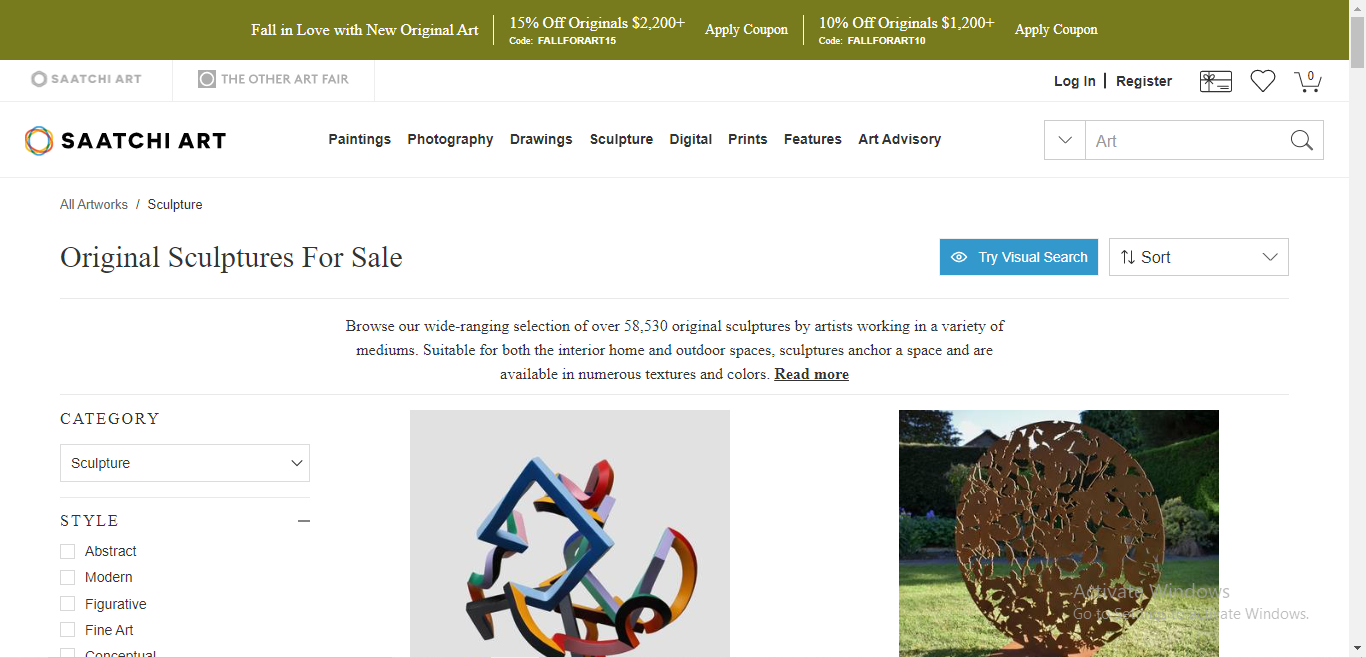
\includegraphics[width = 16cm, height = 9cm]{Saatchi.PNG}
	    \renewcommand{\thefigure}{2.1}
	    \caption{The data of each product is scrapped from this website \textbf{"Saatchi"}}
    \end{figure} 
     \begin{figure}[ht!]
	    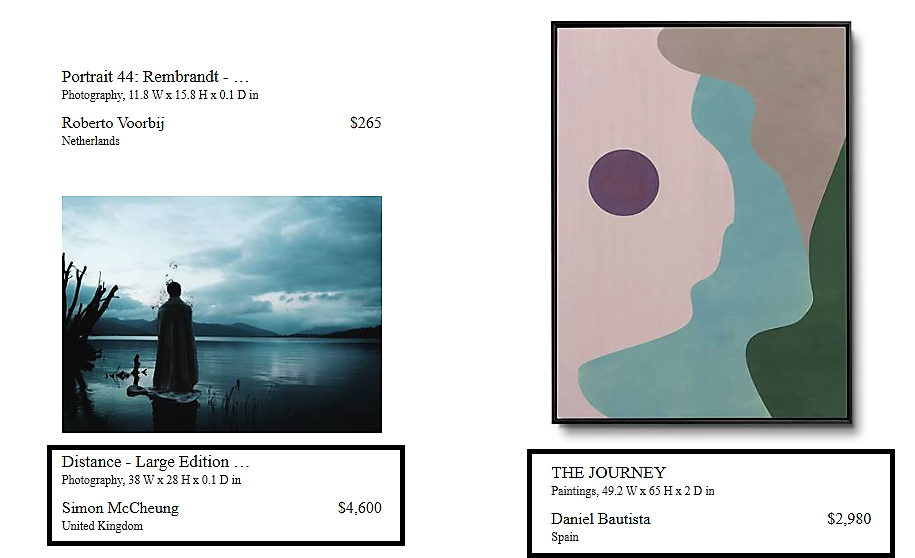
\includegraphics[width = 16cm, height = 9cm]{Attributes.png}
	    \renewcommand{\thefigure}{2.2}
	    \caption{The text in the boxes are the attributes that will be scrapped from this website.}
    \end{figure}
    \newpage
    
    \color{black}\subsubsection{Attributes of Entity(Minimum seven attributes/rows can be increased)}
    \begin{table}[ht!]
    \begin{tabular}{|l|l|l|}
    \hline
    \textbf{Name}          & \textbf{Data Type} & \textbf{Description}                                                                                                                           \\ \hline
    \textbf{Painting Name} & string             & \begin{tabular}[c]{@{}l@{}}contains the name of the \\  product.\end{tabular}                                                                  \\ \hline
    \textbf{Width}         & float              & \begin{tabular}[c]{@{}l@{}}contains the height of the \\  product\end{tabular}                                                                 \\ \hline
    \textbf{Height}        & float              & \begin{tabular}[c]{@{}l@{}}contains the width of the\\  product\end{tabular}                                                                   \\ \hline
    \textbf{Depth}         & float              & \begin{tabular}[c]{@{}l@{}}contains the depth of the canvas\\  on which the product is made .\end{tabular}                                     \\ \hline
    \textbf{Painter}       & string             & \begin{tabular}[c]{@{}l@{}}contains the name of the painter\\  of the painting\end{tabular}                                                    \\ \hline
    \textbf{Category}      & string             & \begin{tabular}[c]{@{}l@{}}tells the category of art; paintings, \\  prints, sculptures, drawings, photography, \\  digitals etc.\end{tabular} \\ \hline
    \textbf{Country}       & string             & \begin{tabular}[c]{@{}l@{}}tells the country of product origin \\  e.g. UK, USA, Pakistan, India, \\  Germany etc.\end{tabular}                \\ \hline
    \textbf{Price}         & int                & \begin{tabular}[c]{@{}l@{}}contains the price of the product\\  in US dollars.\end{tabular}                                                    \\ \hline
    \end{tabular}
    \end{table}
    
    \newpage
    \subsubsection{Searching Filters for each Data Type}
    \begin{table}[ht!]
    \begin{tabular}{|l|l|}
    \hline
    \textbf{Data Type} & \textbf{Filters of this Data Type}                                                                                                                                                                                                                                                                                                                                                                                                                   \\ \hline
    \textbf{Category}  & \begin{tabular}[c]{@{}l@{}}We can display different type of products by applying search on string \\ data type of  "Category". There are 6 type of categories; Paintings, \\ Prints, Photography, Digitals, Sculptures and Drawings. Whenever\\ a specific category button click event is raised, a search is applied on\\ Category column to filter out the object of only those products whose\\ button has been pressed.\end{tabular}             \\ \hline
    \textbf{Country}   & \begin{tabular}[c]{@{}l@{}}We can display different type of products by applying search on string\\ data type of "Country". There are 18 type of countries; United Kingdom,\\ Pakistan, India, China, France, Germany etc.Whenever a specific country\\ button click event is raised , a search is applied on Country column to \\ filter out the object of only those products whose button has been pressed.\end{tabular}                          \\ \hline
    \textbf{Price}     & \begin{tabular}[c]{@{}l@{}}We can display different type of products by applying search on int \\ data type of "Price". There are 6 type of price ranges; Under $500, $500\\ - $1000, $1000 - $2000, $2000 - $5000, $5000 - $10000 and Over $10000.\\ Whenever a specific price button click event is raised , a search is applied \\ on Price column to filter out the object of only those products whose \\ button has been pressed.\end{tabular} \\ \hline
    \end{tabular}
    \end{table}
    
    \subsubsection{Comparison-Based Sorting Algorithms}
    \newpage
    \begin{table}[ht!]
    \begin{tabular}{|l|l|}
    \hline
    \textbf{Algorithm Name}                                           & \textbf{Description(Each algorithm in 2-3 lines)}                                                                                                                                                                                                                                                                                                                                                                                                                   \\ \hline
    \textbf{\begin{tabular}[c]{@{}l@{}}Insertion\\ Sort\end{tabular}} & \begin{tabular}[c]{@{}l@{}}It is an in-place comparison-based sorting where there is a sorted part and \\ an unsorted part in the array. A key is chosen from the array and placed \\ in the array such that it becomes part of the sorted region and this \\ algorithm continues until whole array becomes sorted. This algorithm is \\ not suitable for large data. Average and worst-case complexities are O(n2).\end{tabular}                                   \\ \hline
    \textbf{\begin{tabular}[c]{@{}l@{}}Merge \\ Sort\end{tabular}}    & \begin{tabular}[c]{@{}l@{}}It works on the divide and conquer policy. It divides the array into equal \\ halves until base case is reached and then combines the array in such a \\ way that it is sorted. It is the best comparison-based algorithm with \\ O(n log n) as the worst-case time complexity.\end{tabular}                                                                                                                                             \\ \hline
    \textbf{\begin{tabular}[c]{@{}l@{}}Selection\\ Sort\end{tabular}} & \begin{tabular}[c]{@{}l@{}}It is an in-place comparison-based sorting where the array is divided into\\ one sorted part (at the left end) and the other unsorted part (at the right \\ end). At first, the sorted array is empty and as the algorithm works, it \\ picks the current smallest element from the unsorted array and places it \\ in the sorted array, until the whole array is sorted. Average and worst-\\ case complexities are O(n2).\end{tabular} \\ \hline
    \textbf{\begin{tabular}[c]{@{}l@{}}Bubble\\ Sort\end{tabular}}    & \begin{tabular}[c]{@{}l@{}}It is a comparison-based sorting algorithm in which adjacent elements are\\ compared and swapped if they are not in sorted order. This algorithm is \\ not useful for sorting large data. Average and worst-case complexities are \\ O(n2).\end{tabular}                                                                                                                                                                                 \\ \hline
    \textbf{\begin{tabular}[c]{@{}l@{}}Quick\\ Sort\end{tabular}}     & \begin{tabular}[c]{@{}l@{}}It partitions a larger array into two sub-arrays where one array contains \\ smaller elements than the value of the pivot selected and the other array \\ contains larger elements than the pivot value. The algorithm calls itself \\ recursively twice to sort the two sub-arrays into one array. It is efficient\\ for large data and its average and worst-case complexities are O(n2).\end{tabular}                                 \\ \hline
    \textbf{\begin{tabular}[c]{@{}l@{}}Tim\\ Sort\end{tabular}}       & \begin{tabular}[c]{@{}l@{}}This algorithm works on both Insertion and Merge Sort principles. Its \\ best-case complexity is O(n) and average and worst-case complexities \\ are O(n log n) which is why it is considered to be the best sorting \\ algorithm.\end{tabular}                                                                                                                                                                                             \\ \hline
    \textbf{\begin{tabular}[c]{@{}l@{}}Cocktail\\ Sort\end{tabular}}  & \begin{tabular}[c]{@{}l@{}}It is a variant of Bubble Sort, the only difference is that bubble sort works\\ from left side to right side of the array while Cocktail sort can move in \\ both directions making itself suitable for large data. Its best-case \\ complexity is O(n) and average and worst-case complexities are O(n2).\end{tabular}                                                                                                                  \\ \hline
    \textbf{\begin{tabular}[c]{@{}l@{}}Shell\\ Sort\end{tabular}}     & \begin{tabular}[c]{@{}l@{}}It is a variant of Insertion Sort, the only difference is that Insertion sort \\ moves an element one position ahead while Shell sort allows us to move\\ an element more than one positions. Its best-case complexity is O(n)\\ and average and worst-case complexities are O(n2).\end{tabular}                                                                                                          \\ \hline
    \textbf{\begin{tabular}[c]{@{}l@{}}Heap\\ Sort\end{tabular}}      & \begin{tabular}[c]{@{}l@{}}It is a comparison-based sorting algorithm similar to selection sort \\ which works on the principle of Binary Heap data structure. In this\\ sorting we find the minimum element from the heap and place it at\\ the beginning of the heap, this process continues until whole heap \\ is sorted. Its best, average and worst-case complexities are O(n log n).\end{tabular}                                                            \\ \hline           
    \end{tabular}
    \end{table}
    
    \newpage
    \subsubsection{Pseudo code, Python code and Application of Insertion Sort}
    \paragraph{Pseudo Code :}
    \begin{verbatim}
        InsertionSort(A)
            for j = 0 to A.length
                key = A[j]
                i = j - 1
                        
                while i >= 0 and A[i] > key:
                    temp = A[i + 1]
                    A[i + 1] = A[i]
                    i = i - 1 
                    A[i + 1] = temp
    \end{verbatim}
    \paragraph{Python Code :}
    \begin{verbatim}
    def InsertionSort(self, p, r, column):
        i = 0
        key = 0

        for j in range(p, r):
            key = getattr(self.dataList[j], column)
            temp = self.dataList[j]
            i = j - 1
                
            while i >= 0 and getattr(self.dataList[i], column) > key:
                temp = self.dataList[i + 1]
                self.dataList[i + 1] = self.dataList[i]
                i = i - 1 
                self.dataList[i + 1] = temp
    \end{verbatim}
    \paragraph{Application on Columns :} 
    This algorithm can be applied on string columns; Name, Artist, Country and Category, float columns; Width, Depth and Height, and int column; Price.
    
    \newpage
    \subsubsection{Pseudo code, Python code and Application of Merge Sort}
    \paragraph{Pseudo Code :}
    \begin{verbatim}
    MergeSort(A, p, r) 
        if p < r:
            q = int((p + r) / 2)
            MergeSort(A, p, q)
            MergeSort(A, q + 1, r)
            Merge(A, p, q, r)

    Merge(A, p, q, r)
            n1 = q - p + 1
            n2 = r - q
    
            Let L[0.... n1] and R[0.... n2] be new arrays 
            
            for i = 0 to n1
                    L[i] = A[p + i]
    
            for j = 0 to n2
                    R[i] = A[q + j + 1])
    
            L[n1] = infinity
            R[n2] = infinity
            
            i = 0
            j = 0
            
            for k = p to r + 1
                    if L[i] < R[j]
                            A[k] = A[i]
                            i = i + 1
                    else:
                            A[k] = A[j]
                            j = j + 1     
    \end{verbatim}
    \paragraph{Python Code :}
    \begin{verbatim}
    def MergeSort(self, p, r, column):
        
        if p < r:
            q = int((p + r) / 2)
            self.MergeSort(p, q, column)
            self.MergeSort(q + 1, r, column)
            self.Merge(p, q, r, column)
    
    
    def Merge(self, p, q, r, column):
        n1 = q - p + 1
        n2 = r - q

        left_array = []
        right_array = []
        
        for i in range(n1):
                left_array.append(self.dataList[p + i])

        for j in range(n2):
                right_array.append(self.dataList[q + j + 1])

        x = artPieces(sys.maxsize, sys.maxsize, sys.maxsize, 
        sys.maxsize, sys.maxsize, sys.maxsize, sys.maxsize, sys.maxsize)
        left_array.append(x)
        right_array.append(x)
        
        i = 0
        j = 0
        
        for k in range (p, r + 1):
                if getattr(left_array[i], column) < getattr(right_array[j], column):
                        self.dataList[k] = left_array[i]
                        i = i + 1
                else:
                        self.dataList[k] = right_array[j]
                        j = j + 1
    \end{verbatim}
    \paragraph{Application on Columns :}
    This algorithm can not be applied on string columns; Name, Artist, Country and Category, because the operator < is not applicable on string.It can be applied on float columns; Width, Depth and Height, and int column; Price.
    
    \newpage
    \subsubsection{Pseudo code, Python code and Application of Selection Sort}
    \paragraph{Pseudo Code :}
    \begin{verbatim}
    SelectionSort(A):
        start = 0
        end = A.length - 1
        length = (end - start) + 1
        
        for i = 0 to length
                min = i
                
                for j = i + 1 to length
                
                        if A[j] < A[min]
                                min = j
                                
                switch A[i] with A[min]
    \end{verbatim}
    \paragraph{Python Code :}
    \begin{verbatim}
    def SelectionSort(self, column):
        start = 0
        end = len(self.dataList) - 1
        length = (end - start) + 1
        
        for i in range(length):
                min = i
                
                for j in range(i + 1, length):
                
                        if getattr(self.dataList[j], column) <
                        getattr(self.dataList[min], column):
                                min = j
                                
                (self.dataList[i], self.dataList[min]) =
                (self.dataList[min], self.dataList[i])
    \end{verbatim}
    \paragraph{Application on Columns :} 
    This algorithm can be applied on string columns; Name, Artist, Country and Category, float columns; Width, Depth and Height, and int column; Price.
    
    \newpage
    \subsubsection{Pseudo code, Python code and Application of Bubble Sort}
    \paragraph{Pseudo Code :}
    \begin{verbatim}
    BubbleSort(A):
        start = 0
        end = A.length - 1
        
        for i = start to end
                    
            for j = start to end
                    
                if A[j] > A[j + 1]
                    swicth A[j] with A[j + 1]
    \end{verbatim}
    \paragraph{Python Code :}
    \begin{verbatim}
    def BubbleSort(self, column):
        start = 0
        end = len(self.dataList) - 1
    
        for i in range(start, end):
                
                for j in range(start, end):
                
                        if getattr(self.dataList[j], column) >
                        getattr(self.dataList[j + 1], column):
                                (self.dataList[j], self.dataList[j + 1])
                                = (self.dataList[j + 1], self.dataList[j])
    \end{verbatim}
    \paragraph{Application on Columns :} 
    This algorithm can be applied on string columns; Name, Artist, Country and Category, float columns; Width, Depth and Height, and int column; Price.
    
    \newpage
    \subsubsection{Pseudo code, Python code and Application of Heap Sort}
    \paragraph{Pseudo Code :}
    \begin{verbatim}
    maxHeapify(A, length, i):

        largest = i
        l = (2 * i) + 1
        r = (2 * i) + 2

        if l < length and A[l] > A[i]
                largest = l

        if r < length and A[r] > A[largest]
                largest = r

        if largest != i
                switch A[largest] with A[i]
                maxHeapify(length, largest, column)

        buildMaxHeapify(A, length, column):
        
                for i= length // 2 down to -1
                        maxHeapify(length, i, column)
        
        HeapSort(A):
        
                length = A.Length
                buildMaxHeapify(length, column)
        
                for i = length - 1 down to 0
                        switch A[i] with A[0]
                        length = length - 1
                        maxHeapify(i, 0, column)
    \end{verbatim}
    \paragraph{Python Code :}
    \begin{verbatim}
    def maxHeapify(self, length, i, column):

        largest = i
        l = (2 * i) + 1
        r = (2 * i) + 2

        if l < length and getattr(self.dataList[l], column) >
        getattr(self.dataList[i], column):
                largest = l

        if r < length and getattr(self.dataList[r], column) >
        getattr(self.dataList[largest], column):
                largest = r

        if largest != i:
                (self.dataList[i], self.dataList[largest]) =
                (self.dataList[largest], self.dataList[i])
                self.maxHeapify(length, largest, column)

    def buildMaxHeapify(self, length, column):

        for i in range(length // 2, -1, -1):
                self.maxHeapify(length, i, column)

    def HeapSort(self, column):

        length = len(self.dataList)
        self.buildMaxHeapify(length, column)

        for i in range(length - 1, 0, -1):
                (self.dataList[i], self.dataList[0]) = (self.dataList[0],
                self.dataList[i])
                length = length - 1
                self.maxHeapify(i, 0, column)
    \end{verbatim}
    \paragraph{Application on Columns :} 
    This algorithm can be applied on string columns; Name, Artist, Country and Category, float columns; Width, Depth and Height, and int column; Price.
    
    \newpage
    \subsubsection{Pseudo code, Python code and Application of Quick Sort}
    \paragraph{Pseudo Code :}
    \begin{verbatim}
    QuickSort(A, p, r)
        if p < r
                q = partition(p, r)
                QuickSort(p, q - 1)
                QuickSort(q + 1, r)

        partition(A, p, r)
                x = A[r]
                i = p - 1
        
                for j = p to r
                        if A[j] <= x:
                                i = i + 1
                                switch A[i] with A[j]
                
                switch A[i + 1] and A[r]
    \end{verbatim}
    \paragraph{Python Code :}
    \begin{verbatim}
    def partition(self, p, r, column):
        x = getattr(self.dataList[r], column)
        i = p - 1

        for j in range(p, r):
                if getattr(self.dataList[j], column) <= x:
                        i = i + 1
                        (self.dataList[i], self.dataList[j]) =
                        (self.dataList[j], self.dataList[i])
        
        (self.dataList[i + 1], self.dataList[r]) = (self.dataList[r],
        self.dataList[i + 1])
        return i + 1


    def QuickSort(self, p, r, column):
        if p < r:
                q = self.partition(p, r, column)
                self.QuickSort(p, q - 1, column)
                self.QuickSort(q + 1, r, column)
    \end{verbatim}
    \paragraph{Application on Columns :} 
    This algorithm can be applied on string columns; Name, Artist, Country and Category, float columns; Width, Depth and Height, and int column; Price.
    
    \subsubsection{Pseudo code, Python code and Application of Genome Sort}
    \paragraph{Pseudo Code :}
    \begin{verbatim}
    GenomeSort(A)
        length = A.Length
        idx = 0 

        while idx < length

                if idx == 0 or A[idx] >= A[idx - 1]
                        idx = idx + 1

                else:
                        switch A[idx] and A[idx - 1])
                        idx = idx - 1
    \end{verbatim}
    \paragraph{Python Code :}
    \begin{verbatim}
    def GenomeSort(self, column):
        length = len(self.dataList)
        idx = 0 

        while idx < length:

                if idx == 0 or getattr(self.dataList[idx], column) >=
                getattr(self.dataList[idx - 1], column):
                        idx = idx + 1

                else:
                        (self.dataList[idx], self.dataList[idx - 1]) =
                        (self.dataList[idx - 1], self.dataList[idx])
                        idx = idx - 1
    \end{verbatim}
    \paragraph{Application on Columns :} 
    This algorithm can be applied on string columns; Name, Artist, Country and Category, float columns; Width, Depth and Height, and int column; Price.
    
    \newpage
    \subsubsection{Pseudo code, Python code and Application of Cocktail Sort}
    \paragraph{Pseudo Code :}
    \begin{verbatim}
    CocktailSort(A)
        length = A.Length

        for i = length - 1 down to 0

                for j = 0 to i
                        if A[j] > A[j + 1]
                                switch A[j] and A[j + 1]

                for j = i down to 0
                        if A[j] < A[j - 1]
                                switch A[j] and A[j - 1]
    \end{verbatim}
    \paragraph{Python Code :}
    \begin{verbatim}
    def CocktailSort(self, column):
        length = len(self.dataList)

        for i in range(length - 1, 0, -1):

                for j in range(i):
                        if getattr(self.dataList[j], column) >
                        getattr(self.dataList[j + 1], column):
                                (self.dataList[j], self.dataList[j + 1])
                                = (self.dataList[j + 1], self.dataList[j])

                for j in range(i, 0, -1):
                        if getattr(self.dataList[j], column) <
                        getattr(self.dataList[j - 1], column):
                                (self.dataList[j], self.dataList[j - 1])
                                = (self.dataList[j - 1], self.dataList[j]) 
    \end{verbatim}
    \paragraph{Application on Columns :} 
    This algorithm can be applied on string columns; Name, Artist, Country and Category, float columns; Width, Depth and Height, and int column; Price.
    
    \newpage
    \subsubsection{Pseudo code, Python code and Application of Shell Sort}
    \paragraph{Pseudo Code :}
    \begin{verbatim}
    ShellSort(A)

        gap = A.Length // 2
     
        while gap > 0
                j = gap
                
                while j < A.Length
                        i = j - gap 
                        
                        while i >= 0
                                
                                if A[i + gap] > A[i]
                                        break
                                else:
                                        switch A[i+gap] and A[i]
                
                                i = i - gap 

                        j = j + 1
                        
                gap = gap // 2
    \end{verbatim}
    \paragraph{Python Code :}
    \begin{verbatim}
    def ShellSort(self, column):

        gap = len(self.dataList)//2
     
        while gap>0:
                j = gap
                
                while j < len(self.dataList):
                        i = j - gap 
                        
                        while i >= 0:
                                
                                if getattr(self.dataList[i + gap],
                                column) > getattr(self.dataList[i],
                                column):
                                        break
                                else:
                                        self.dataList[i+gap],
                                        self.dataList[i] =
                                        self.dataList[i],
                                        self.dataList[i+gap]
                
                                i = i - gap 

                        j = j + 1
                        
                gap = gap // 2
    \end{verbatim}
    \paragraph{Application on Columns :} 
    This algorithm can be applied on string columns; Name, Artist, Country and Category, float columns; Width, Depth and Height, and int column; Price.
    
    \subsubsection{Pseudo code, Python code and Application of Tim Sort}
    \paragraph{Pseudo Code :}
    \begin{verbatim}
    TimSort(A)
        length = A.Length
        minRun = 32

        for p = 0 to A.Length
                r = minimun of (p + minRun - 1, length -1)
                InsertionSort(p, r)

        size = minRun
        while size < length
                for p in range(0, length, 2 * size):
                        q = minimum of (length - 1, p + size - 1)
                        r = mininimum of ((p + 2 * size - 1), (length -
                        1))

                        if q < r:
                                Merge(p, q, r, column)        

                size = 2 * size
    \end{verbatim}
    \paragraph{Python Code :}
    \begin{verbatim}
    def TimSort(self, column):
        length = len(self.dataList)
        minRun = 32

        for p in range(0, length, minRun):
                r = min(p + minRun - 1, length -1)
                self.InsertionSort(p, r, column)

        size = minRun
        while size < length:
                for p in range(0, length, 2 * size):
                        q = min(length - 1, p + size - 1)
                        r = min((p + 2 * size - 1), (length - 1))

                        if q < r:
                                self.Merge(p, q, r, column)        

                size = 2 * size
    \end{verbatim}
    \paragraph{Application on Columns :} 
    This algorithm can not be applied on string columns; Name, Artist, Country and Category, because the operator < is not applicable on string.It can be applied on float columns; Width, Depth and Height, and int column; Price.
    
    \newpage
    \subsubsection{Non-Comparison-Based Sorting Algorithms}
    \begin{table}[ht!]
    \begin{tabular}{|l|l|}
    \hline
    \textbf{Algorithm Name}                                            & \textbf{Description(Each algorithm in 2-3 lines)}                                                                                                                                                                                                                                                                                                                                                           \\ \hline
    \textbf{\begin{tabular}[c]{@{}l@{}}Counting\\ Sort\end{tabular}}   & \begin{tabular}[c]{@{}l@{}}It is a non-comparison-based sorting algorithm where we evaluate the\\ maximum number in the array and make a count array of the maximum \\ number. Every number is placed at its index i.e (0 at 0), increasing \\ count by one and then we sort the array accordingly.\end{tabular}                                                                                            \\ \hline
    \textbf{\begin{tabular}[c]{@{}l@{}}Bucket\\ Sort\end{tabular}}     & \begin{tabular}[c]{@{}l@{}}It puts the elements of an array into buckets (which are themselves an \\ array) and then each bucket is sorted by any other sort i.e (Insertion \\ Sort).\end{tabular}                                                                                                                                                                                                          \\ \hline
    \textbf{\begin{tabular}[c]{@{}l@{}}Radix\\ Sort\end{tabular}}      & \begin{tabular}[c]{@{}l@{}}It is a variant of counting sort, the only difference is that if there is an \\ element 1000 in the array, counting sort would make an array of 1000\\ elements while radix sort will create only 10 buckets for digits 0-9 \\ and then it applies counting sort from least significant integer to most\\ significant integer and the end sorted array is returned.\end{tabular} \\ \hline
    \textbf{\begin{tabular}[c]{@{}l@{}}PigeonHole\\ Sort\end{tabular}} & \begin{tabular}[c]{@{}l@{}}It is similar to counting sort. It initially moves data to buckets and then \\ to their desired positions to sort the array.\end{tabular}                                                                                       \\ \hline
    \end{tabular}
    \end{table}
    
    \subsubsection{Searching Algorithms}
    \begin{table}[ht!]
    \begin{tabular}{|l|l|}
    \hline
    \textbf{\begin{tabular}[c]{@{}l@{}}Linear\\ Search\end{tabular}}         & \begin{tabular}[c]{@{}l@{}}It is a search in which a loop executes over the whole data of a column\\ selected and  if any object matches the specific condition statement, \\ it is returned and vice versa. This actually filters out information for\\ users.\end{tabular}                                              \\ \hline
    \textbf{\begin{tabular}[c]{@{}l@{}}Start\\ Letter\\ Search\end{tabular}} & \begin{tabular}[c]{@{}l@{}}It is a search in which the user enters an alphabetic letter from A to Z \\ and a loop executes over the whole data of a selected column, if an \\ object's first letter is equal to the condition given, it is returned and \\ vice versa. This also works as a filter for data.\end{tabular} \\ \hline
    \textbf{\begin{tabular}[c]{@{}l@{}}Middle\\ Word\\ Search\end{tabular}}  & \begin{tabular}[c]{@{}l@{}}It is a search in which the user enters a word and a loop executes over\\ the whole data of a selected column, if an object contains that word \\ which is given in the condition then it is returned and vice versa. It is \\ a searching filter too.\end{tabular}                            \\ \hline
    \end{tabular}
    \end{table}
    
    \newpage
    \subsubsection{Pseudo code, Python code and Application of Counting Sort}
    \paragraph{Pseudo Code :}
    \begin{verbatim}
    CountingSort(A, B, max, column)

        Let C[] be a list
        Let Result[] be a list

        for i = 0 to max
                append 0 in C

        for j = 0 to A.Length
                C[A[j]] = C[A[j]] + 1

        for i = 1 to max
                C[i] = C[i] + C[i - 1]

        for j = A.Length down to  0 
                B[(C[A[j-1]]) - 1] =  A[j - 1]      
                C[A[j - 1]] = C[A[j - 1]] - 1

        for i = 0 to A.Length
                A[i] = B[i]
    \end{verbatim}
    \paragraph{Python Code :}
    \begin{verbatim}
    def CountingSort(self, B, max, column):

        C = []
        Result = []

        for i in range (max):
                C.append(0)

        for j in range (len(self.dataList)):
                C[getattr(self.dataList[j], column)] =
                C[getattr(self.dataList[j], column)] + 1

        for i in range (1, max):
                C[i] = C[i] + C[i - 1]

        for j in range (len(self.dataList), 0 , -1):
                B[(C[getattr(self.dataList[j-1], column)]) - 1] =
                self.dataList[j - 1]      
                C[getattr(self.dataList[j - 1], column)] =
                C[getattr(self.dataList[j - 1], column)] - 1

        for i in range (len(self.dataList)):
                self.dataList[i] = B[i]
    \end{verbatim}
    \paragraph{Application on Columns :} 
    This algorithm can only be applied on int column; Price, as we put integers on their specific index which are discrete values thus float and string columns cannot be sorted by this algorithm.
    
    \newpage
    \subsubsection{Pseudo code, Python code and Application of Bucket Sort}
    \paragraph{Pseudo Code :}
    \begin{verbatim}
        BucketSort(A)
        Let B[] be a List
        n = len(A)

        for i = 0 to (n)
                B.append([])

        for i = 0 to n
                B[int(n * A[i])].append(A[i])

        for i = 0 to n
                B[i] = BucketInsertionSort(B[i])

        B = np.concatenate(B)

    \end{verbatim}
    \paragraph{Python Code :}
    \begin{verbatim}
    def BucketInsertionSort(self, array):
        i = 0
        key = 0

        for j in range(1, len(array)):
                key = array[j]
                i = j - 1
        
                while i >= 0 and array[i] > key:
                        array[i+1] = array[i]
                        i = i - 1 
                        array[i + 1] = key


    def BucketSort(self, column):
        B = []
        n = len(column)

        for i in range (n):
                B.append([])

        for i in range (n):
                B[int(n * getattr(self.dataList[i],
                column))].append(self.dataList[i])

        for i in range (n):
                B[i] = self.BucketInsertionSort(B[i])

        B = np.concatenate(B)
    \end{verbatim}
    \paragraph{Application on Columns :} 
    This algorithm can only be applied on float columns; Width, Height and Depth, but int and string columns have a different orientation thus it cannot be applied on them.
    
    \subsubsection{Pseudo code, Python code and Application of Radix Sort}
    \paragraph{Pseudo Code :}
    \begin{verbatim}
    RadixSort(A)
        d = -1

        for i = 0 to A.Length
                if d > A[i]
                        d = A[i]

        B = [0 for i = 0 to A.Length]
        n = 1
        while (d // n > 0)
                A = RadixCountingSort(B, n, column) 
                n = n * 10
    \end{verbatim}
    \paragraph{Python Code :}
    \begin{verbatim}
    def RadixCountingSort(self, B, n, column):
        C = [0] * 10

        for j in range (len(self.dataList)):
                temp = getattr(self.dataList[j], column) // n
                C[temp % 10] = C[temp % 10] + 1

        for i in range (1, 10):
                C[i] = C[i] + C[i - 1]

        i = len(self.dataList) - 1
        while (i >= 0):
                temp = getattr(self.dataList[i], column) // n 
                B[C[temp % 10] - 1] = self.dataList[i]
                C[temp % 10] = C[temp % 10] - 1
                i = i - 1

        for i in range (len(self.dataList)):
                self.dataList[i] = B[i]
        return self.dataList


    def RadixSort(self, column):
        d = -1

        for i in range(0, len(self.dataList)):
                if d > getattr(self.dataList[i], column):
                        d = getattr(self.dataList[i], column)

        B = [0 for i in range(len(self.dataList))]
        n = 1
        while (d // n > 0):
                self.dataList = self.RadixCountingSort(B, n, column)
                n = n * 10
    \end{verbatim}
    \paragraph{Application on Columns :} 
    This algorithm can only be applied on int column; Price, as we put integers on their specific index which are discrete values thus float and string columns cannot be sorted by this algorithm.
    
    \newpage
    \subsubsection{Pseudo code, Python code and Application of PigeonHole Sort}
    \paragraph{Pseudo Code :}
    \begin{verbatim}
    PigeonHoleSort(A)
        Smallest = 9999999999
        Largest = -1

        for i = 0 to A.Length
                if Smallest > A[i]
                        Smallest = A[i]

        for i = 0 to A.Length
                if Largest < A[i]
                        Largest = A[i]

        
        NumberOfHoles = Largest - Smallest + 1
        Holes = []

        for i = 0 to NumberOfHoles)
                Holes.append(0)

        for j = 0 to A.Length
                Holes[j - Smallest] = Holes[j - Smallest] + 1

        clear array A
        for x = 0 to NumberOfHoles
                while (Holes[x] > 0)
                        Holes[x] = Holes[x] - 1
                        A.append(x + Smallest)
    \end{verbatim}
    \paragraph{Python Code :}
    \begin{verbatim}
    def PigeonHoleSort(self, column):
        Smallest = 9999999999
        Largest = -1

        for i in range(0, len(self.dataList)):
                if Smallest > getattr(self.dataList[i], column):
                        Smallest = getattr(self.dataList[i], column)

        for i in range(0, len(self.dataList)):
                if Largest < getattr(self.dataList[i], column):
                        Largest = getattr(self.dataList[i], column)

        
        NumberOfHoles = Largest - Smallest + 1
        Holes = []

        for i in range (NumberOfHoles):
                Holes.append(0)

        for j in self.dataList:
                Holes[j - Smallest] = Holes[j - Smallest] + 1

        self.dataList.clear()
        for x in range (NumberOfHoles):
                while (Holes[x] > 0):
                        Holes[x] = Holes[x] - 1
                        self.dataList.append(x + Smallest)
    \end{verbatim}
    \paragraph{Application on Columns :} 
     This algorithm can only be applied on int column; Price, as we put integers on their specific index which are discrete values thus float and string columns cannot be sorted by this algorithm.
    
    \newpage
    \subsubsection{Pseudo code, Python code and Application of Linear Search}
    \paragraph{Pseudo Code :}
    \begin{verbatim}
    LinearSearch(A, B, search)
        for i = 0 to A.Length
                        if A[i] == search
                                B.append(A[i])
    \end{verbatim}
    \paragraph{Python Code :}
    \begin{verbatim}
    def LinearSearch(self, search, column):

        if column == "Width" or column == "Height" or column == "Depth":
                search = float(search)

        elif column == "Price":
                search = int(search)

        for i in range(0, len(self.dataList)):
                        if getattr(self.dataList[i], column) == search:
                            self.searchList.append(self.dataList[i]))
    \end{verbatim}
    \paragraph{Application on Columns :} 
    This algorithm can be applied on string columns; Name, Artist, Country and Category, float columns; Width, Depth and Height, and int column; Price.
    
    \newpage
    \subsubsection{Pseudo code, Python code and Application of Start Letter Search}
    \paragraph{Pseudo Code :}
    \begin{verbatim}
    StartLetterSeacrh(A, B, search)
        for i = 0 to A.Length
                
                if attribute[0] == search
                        B.append(A[i])
    \end{verbatim}
    \paragraph{Python Code :}
    \begin{verbatim}
     def StartLetterSeacrh(self, search, column):
        length = len(self.dataList)

        for i in range(0, length):
                if column == "Width" or column == "Height" or column ==
                "Depth" or column == "Price":
                        attribute = getattr(self.dataList[i], column)
                        attribute = str(attribute)

                else:
                        attribute = getattr(self.dataList[i], column)

                if attribute[0] == search:
                        self.searchList.append(self.dataList[i])
    \end{verbatim}
    \paragraph{Application on Columns :} 
    This algorithm can be applied on string columns; Name, Artist, Country and Category, float columns; Width, Depth and Height, and int column; Price.
    
    \newpage
    \subsubsection{Pseudo code, Python code and Application of Middle Word Search}
    \paragraph{Pseudo Code :}
    \begin{verbatim}
    MiddleWordsSearch(A, B, search)

        for i = 0 to A.Length
                
                attribute = A[i]
                wordList = attribute.split()

                for j = 0 to wordList.Length
                        if wordList[j] == search
                                B.append(A[i])
    \end{verbatim}
    \paragraph{Python Code :}
    \begin{verbatim}
    def MiddleWordsSearch(self, search, column):

        for i in range(0, len(self.dataList)):
                
                attribute = getattr(self.dataList[i], column)
                wordList = attribute.split()

                for j in range(0, len(wordList)):
                        if wordList[j] == search:
                            self.searchList.append(self.dataList[i])
    \end{verbatim}
    \paragraph{Application on Columns :} 
    This algorithm can be applied on string columns; Name, Artist, Country but not Category because this column has one word which cannot be split. It cannot be applied on float columns; Width, Height, Depth and int column; Price because they both cannot be split.
    
    \subsection{Scrapping Code}
    \begin{verbatim}
from selenium import webdriver
from bs4 import BeautifulSoup
import pandas as pd
from csv import writer

path = 'C:\Program Files\chromedriver_win32\chromedriver.exe'
driver = webdriver.Chrome(path)

next="/paintings?hitsPerPage=100"

with open('PaintingsData.csv', "w", encoding='utf8', newline='') as f:
    
    thewriter =  writer(f)
    header = ['Name', 'Width', 'Height', 'Depth', 'Painter',
    'Country','Price']
    thewriter.writerow(header)

    for i in range(250):

        driver.get("https://www.saatchiart.com" + next)
        content = driver.page_source
        soup = BeautifulSoup(content)

        page1 = soup.findAll('div',attrs={'class':'sc-15ws6ki-0 wZWfg'})
        link = soup.find('a',attrs={'title':'Next'})
        next=link['href']

        for i in page1:

            a = i.find('div',attrs={'data-type':'artwork-info'})
            b = i.find('div',attrs={'data-type':'artist-info'})
            c = i.find('div',attrs={'data-type':'prices'})
            d = b.findAll('p')
            
            name= a.p.a.text
            size= a.find('span',attrs={'class':'sc-144xit5-0 juFwTn'})
            size = size.text
            data = size.split(" ")
            width = data[0]
            height = data[3]
            depth = data[6]
            painter = b.p.a.text
            price = c.p.text
            country = d[1].text
            info = [name, width, height, depth, painter, country, price]
            thewriter.writerow(info)
    \end{verbatim}
    
    \newpage
    \section{Interfaces of Project}
    \subsection{GUI}
    \begin{figure}[ht!]
	    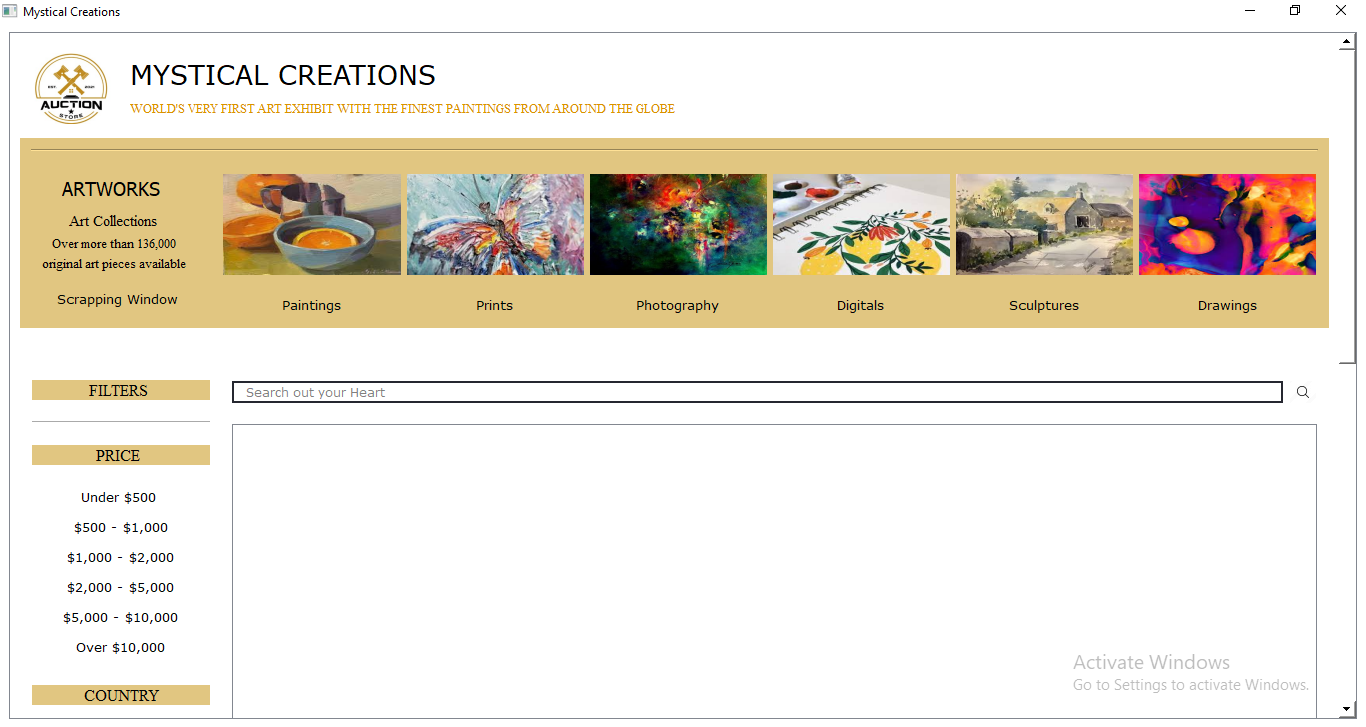
\includegraphics[width = 16cm, height = 9cm]{Unloaded Data.PNG}
	    \renewcommand{\thefigure}{3.1}
	    \caption{Interface of Project with Data not Imported Yet}
    \end{figure}
    \begin{figure}[ht!]
	    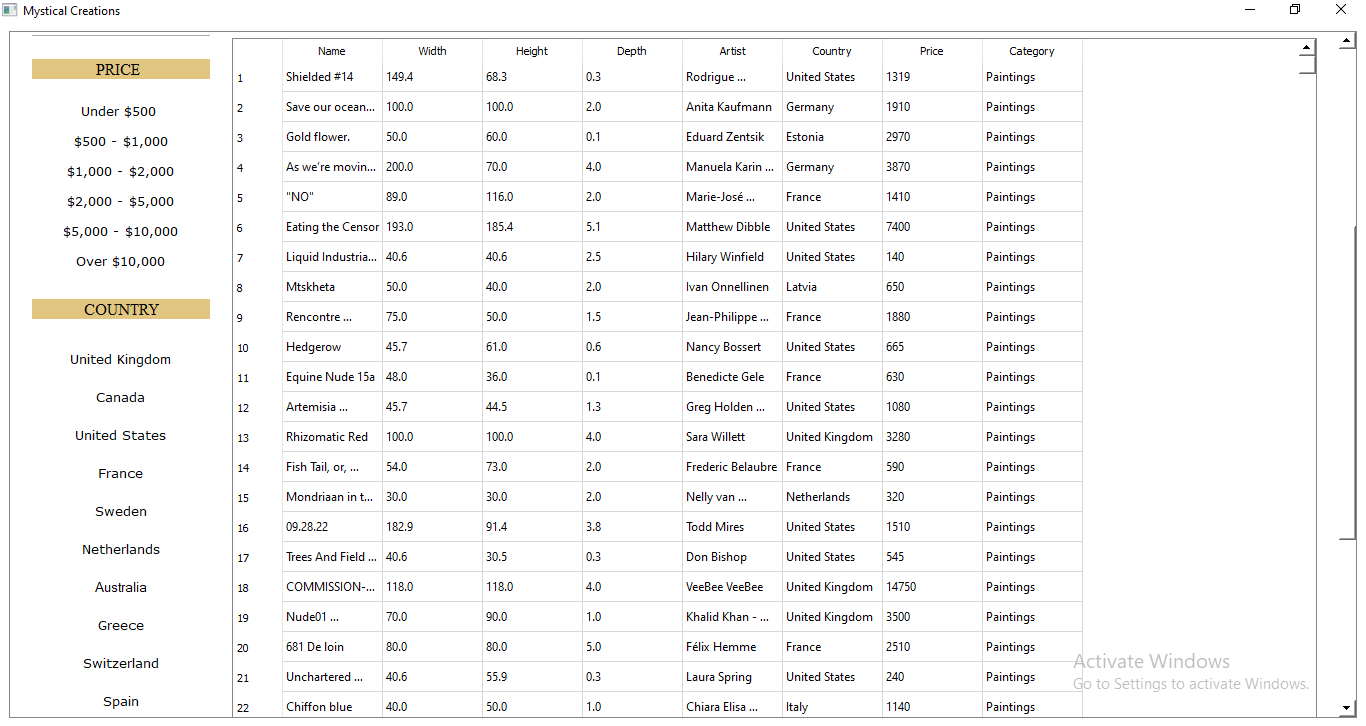
\includegraphics[width = 16cm, height = 9cm]{Imported Data.PNG}
	    \renewcommand{\thefigure}{3.2}
	    \caption{Interface of Project with Imported Data}
    \end{figure}
    
    \newpage
    \begin{figure}[ht!]
	    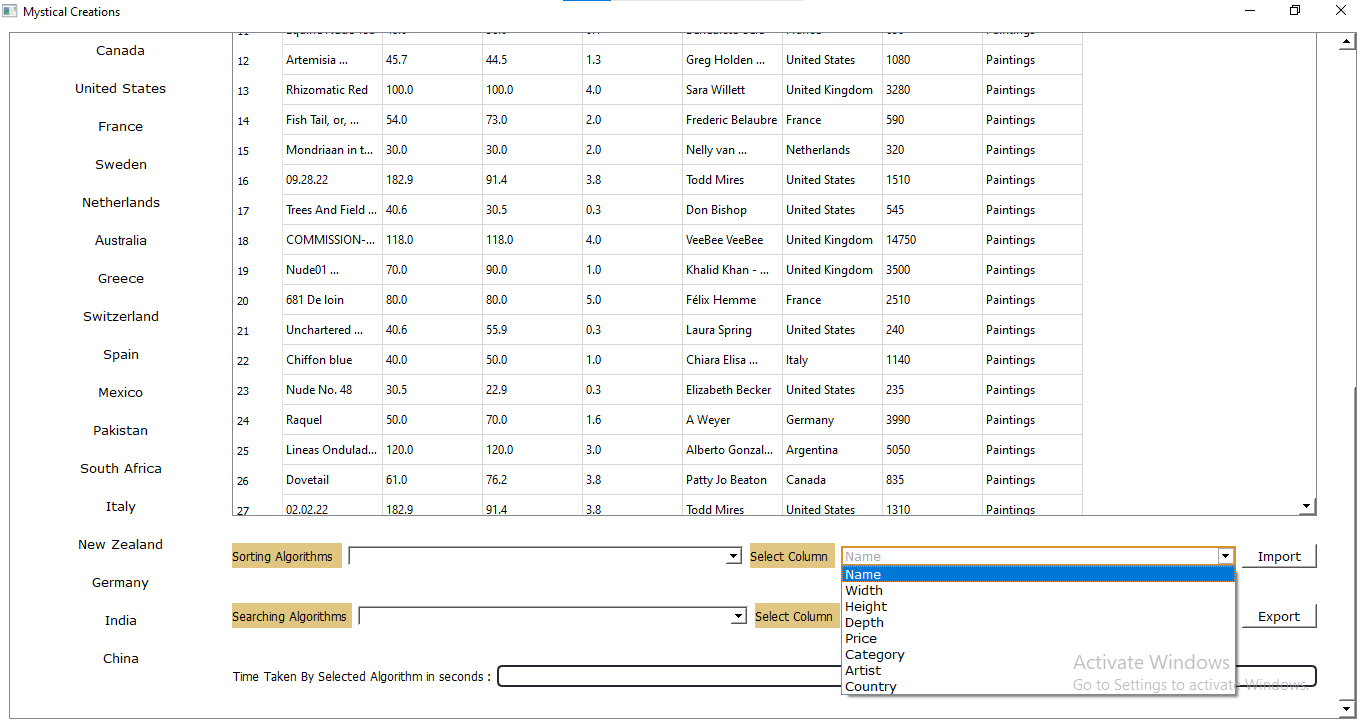
\includegraphics[width = 16cm, height = 9cm]{Columns.png}
	    \renewcommand{\thefigure}{3.3}
	    \caption{Columns in the Table Widget on which sorting and searching algorithms are applied}
    \end{figure}
    \begin{figure}[ht!]
	    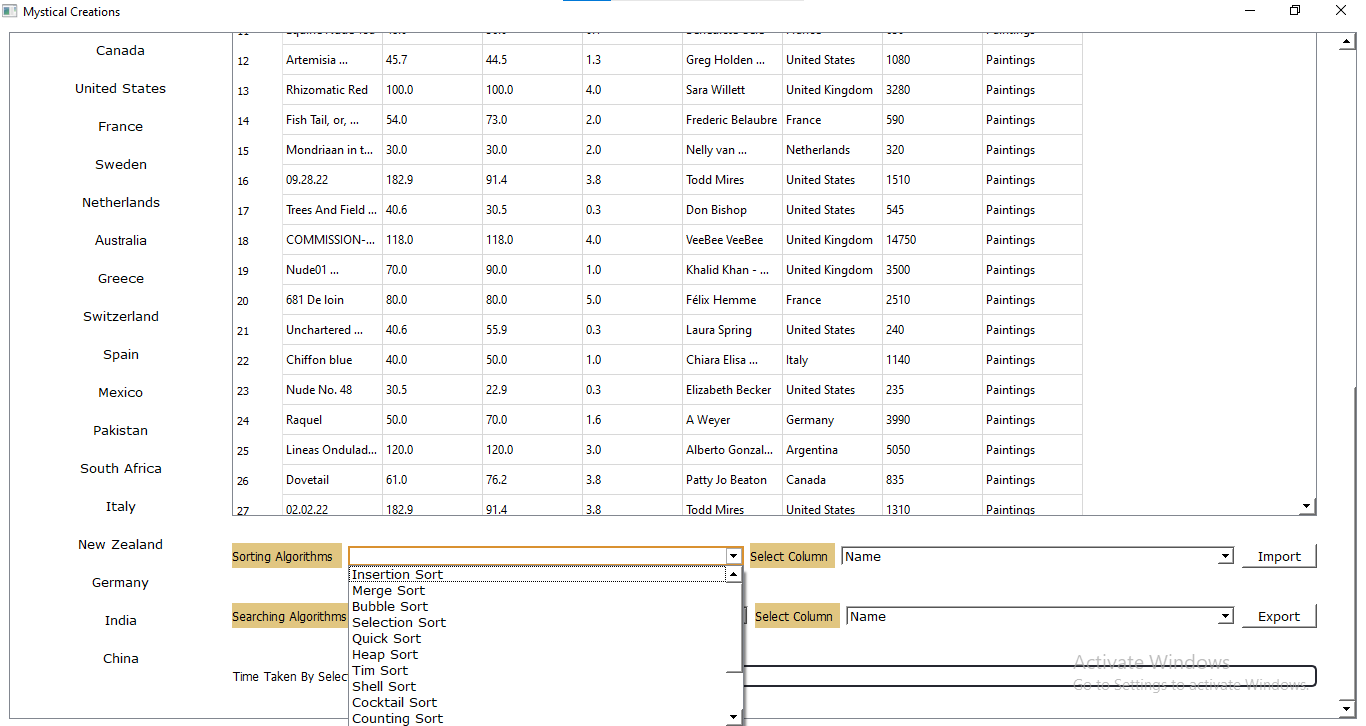
\includegraphics[width = 16cm, height = 9cm]{Sorting Algorithms.png}
	    \renewcommand{\thefigure}{3.4}
	    \caption{There are 14 types of Sorting Algorithms in our project}
    \end{figure}
    
    \newpage
    \begin{figure}[ht!]
	    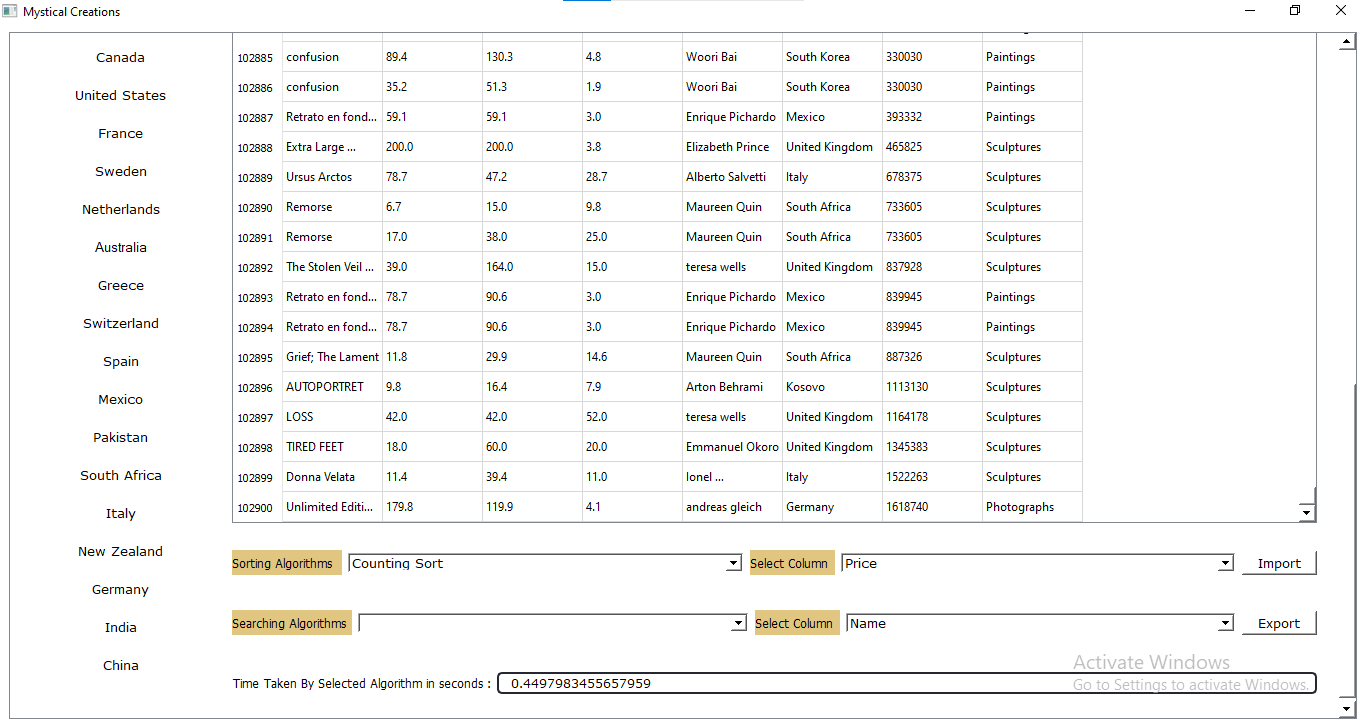
\includegraphics[width = 16cm, height = 9cm]{Sorted Data.png}
	    \renewcommand{\thefigure}{3.5}
	    \caption{Data in Table Widget after Sorting is applied}
    \end{figure}
    \begin{figure}[ht!]
	    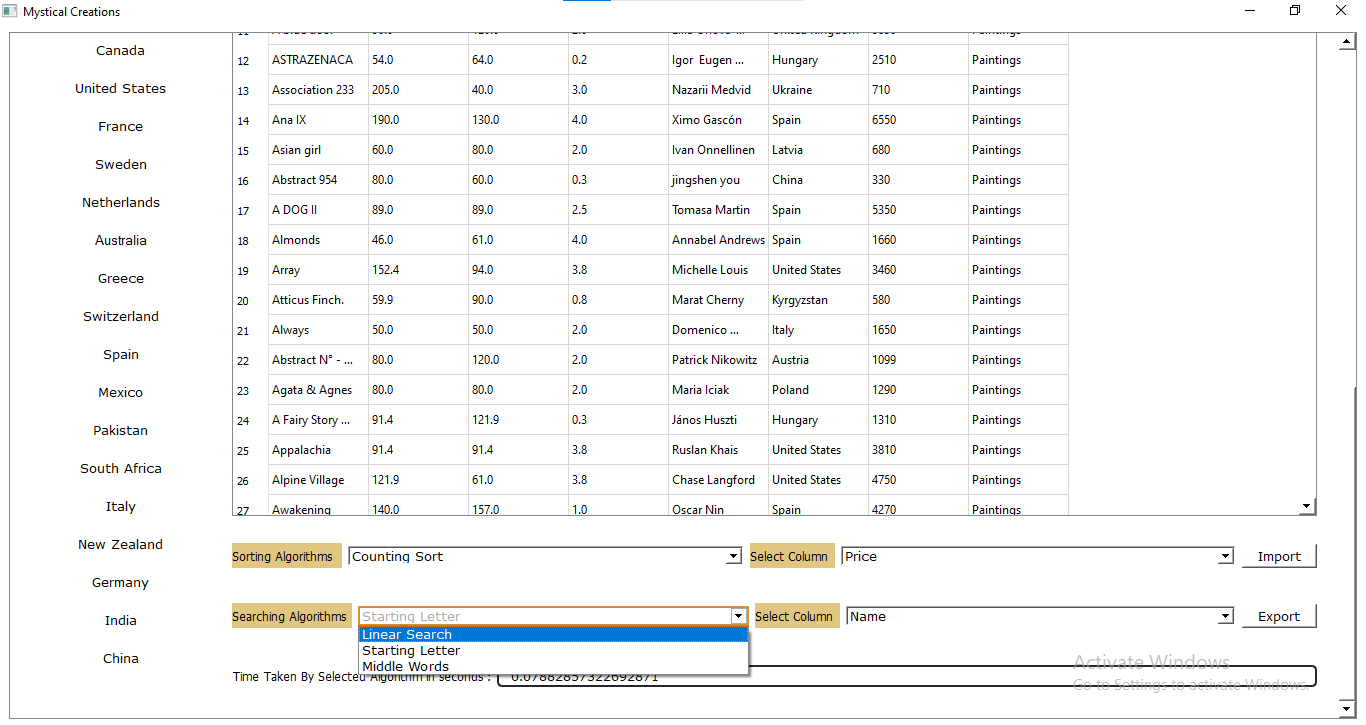
\includegraphics[width = 16cm, height = 9cm]{Searching Algorithms.png}
	    \renewcommand{\thefigure}{3.6}
	    \caption{There are 3 types of Searching Algorithms in our project}
    \end{figure}
    
    \newpage
    \begin{figure}[ht!]
	    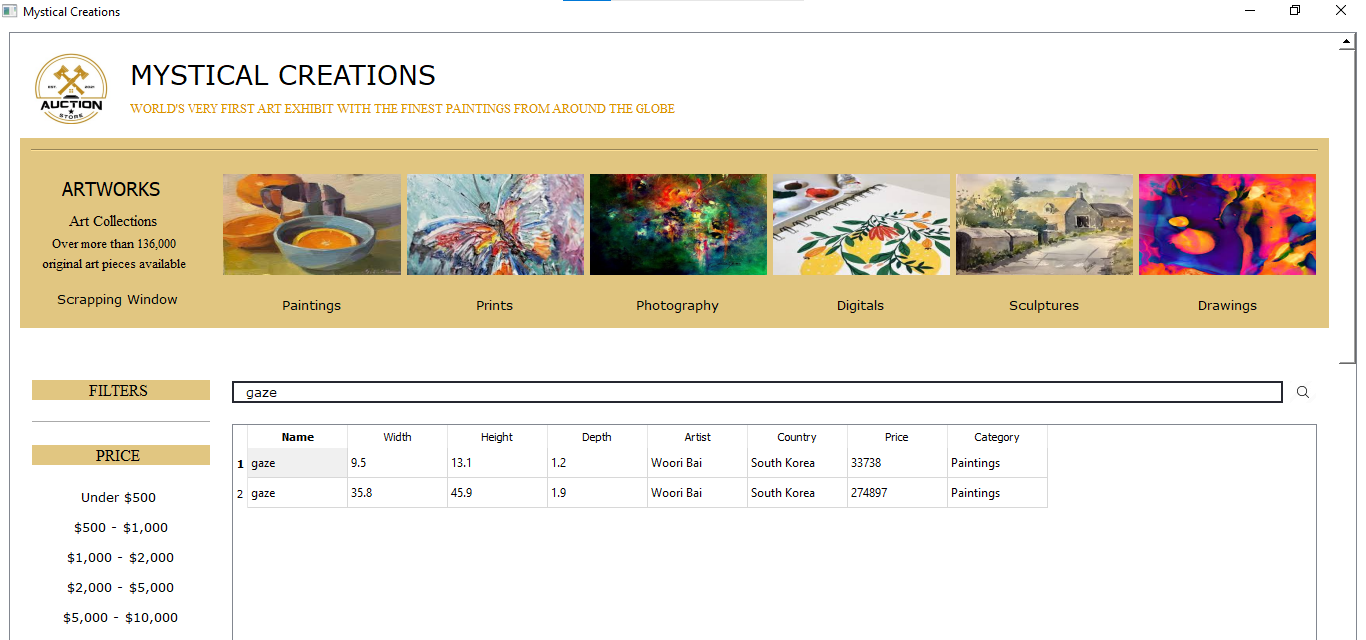
\includegraphics[width = 16cm, height = 9cm]{Searched Data.png} 
	    \renewcommand{\thefigure}{3.7}
	    \caption{Data in Table Widget after Linear Searching is applied}
    \end{figure}
    \begin{figure}[ht!]
	    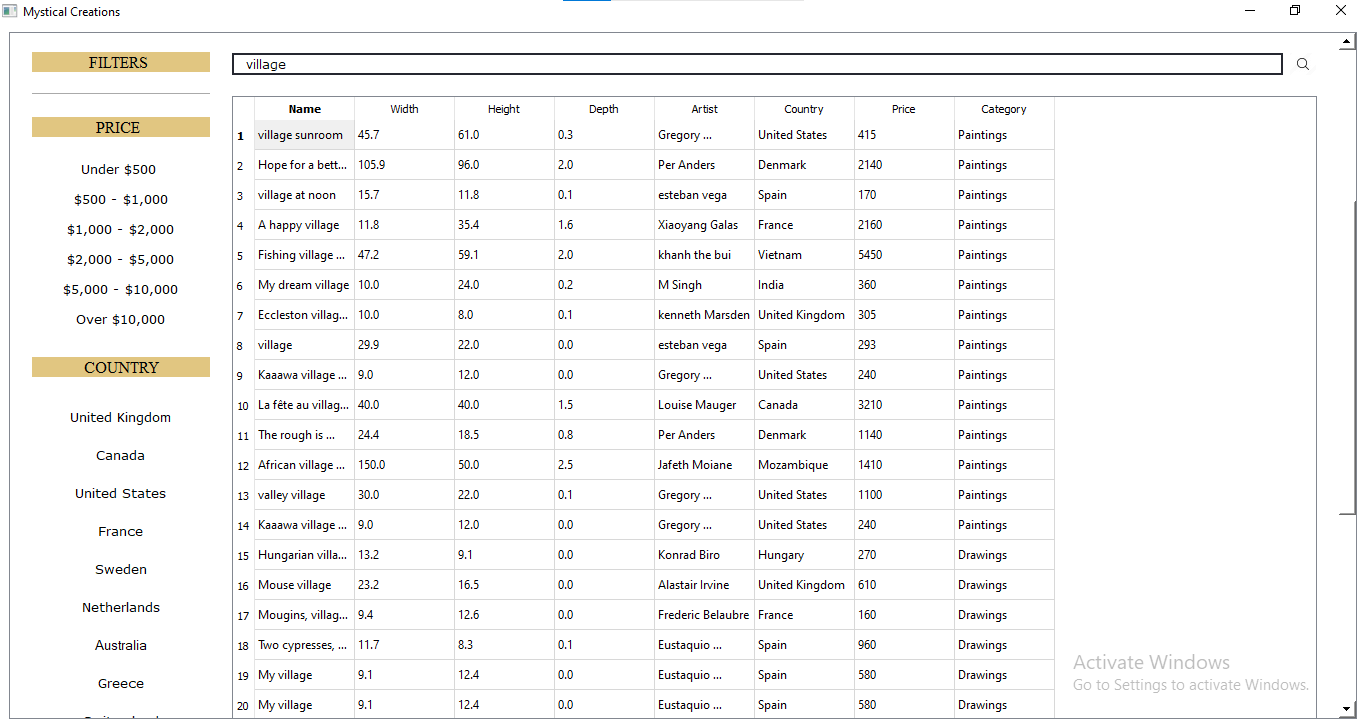
\includegraphics[width = 16cm, height = 9cm]{Middle Words Search.png}
	    \renewcommand{\thefigure}{3.8}
	    \caption{Results of middle word search}
    \end{figure}
    
    \newpage
    \begin{figure}[ht!]
	    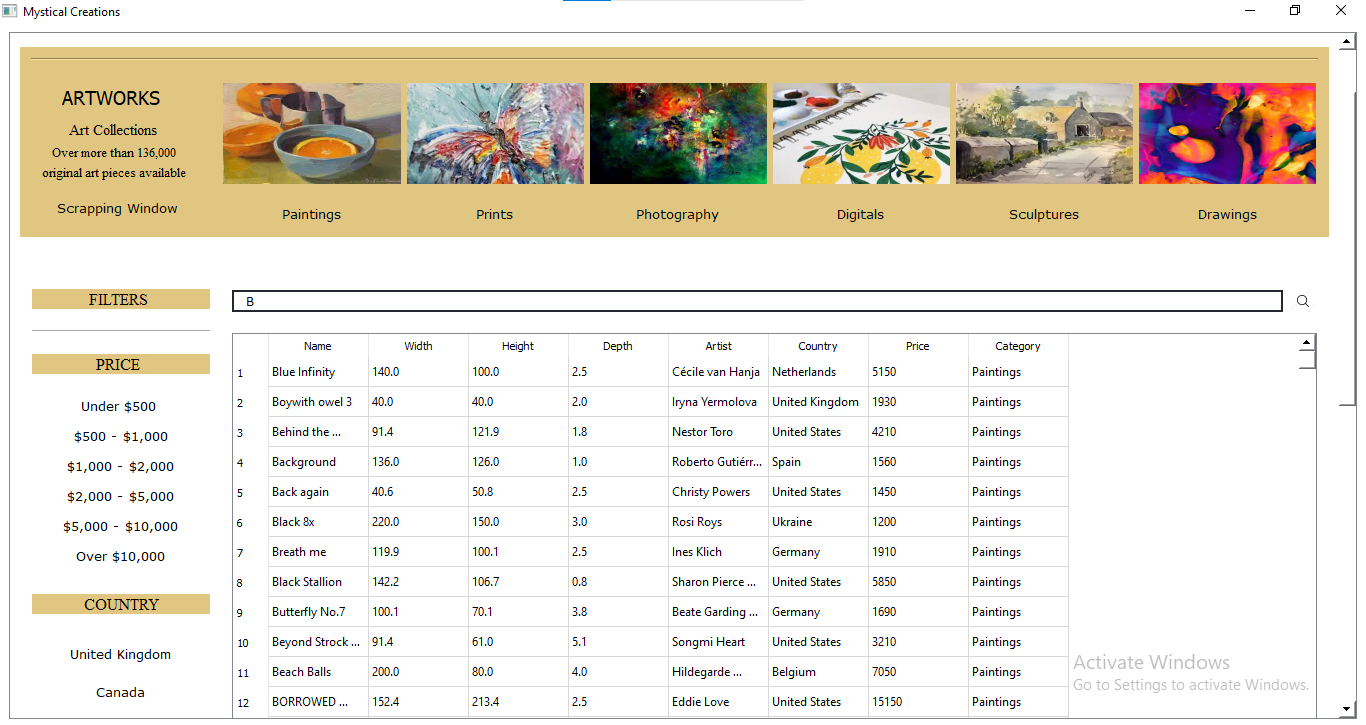
\includegraphics[width = 16cm, height = 9cm]{Starting Letter Search.png}
	    \renewcommand{\thefigure}{3.9}
	    \caption{Results of Starting Letter Search}
    \end{figure}
    \begin{figure}[ht!]
	    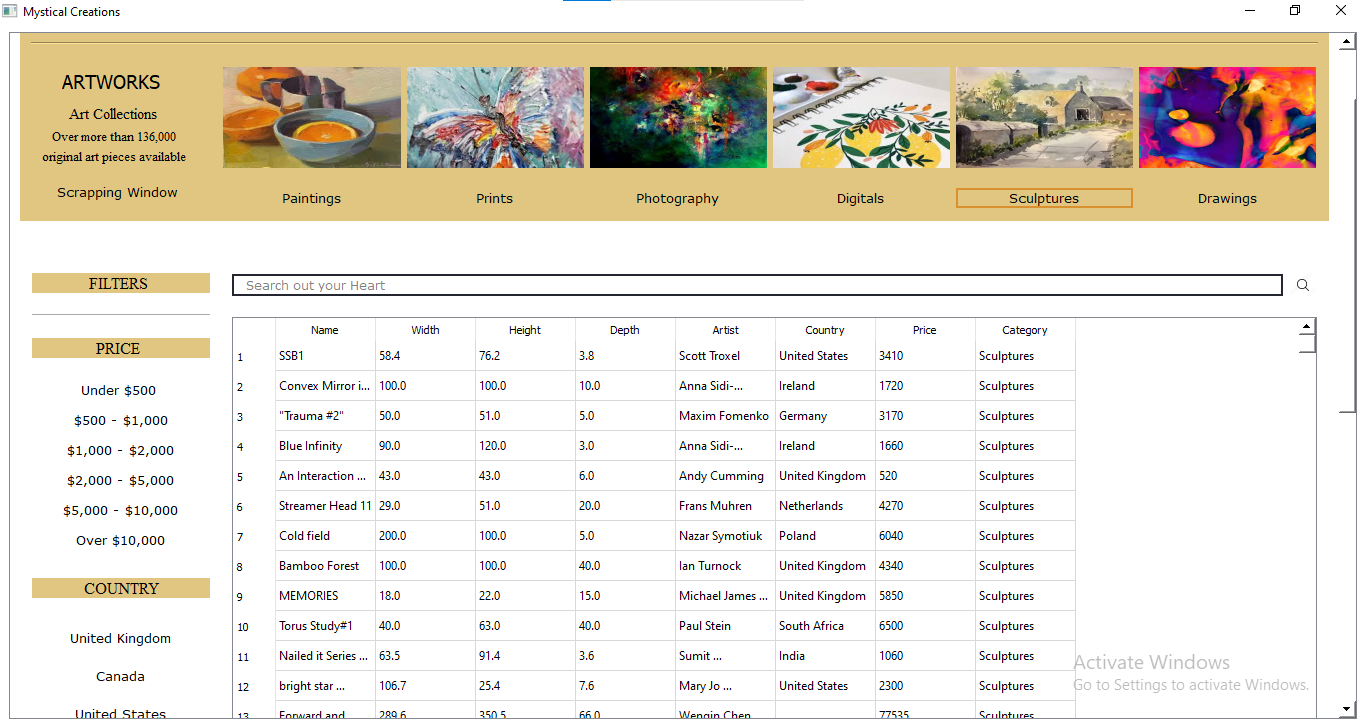
\includegraphics[width = 16cm, height = 9cm]{Category Filters.png}
	    \renewcommand{\thefigure}{3.10}
	    \caption{Data after Category filter is applied}
    \end{figure}
    
    \newpage
    \begin{figure}[ht!]
	    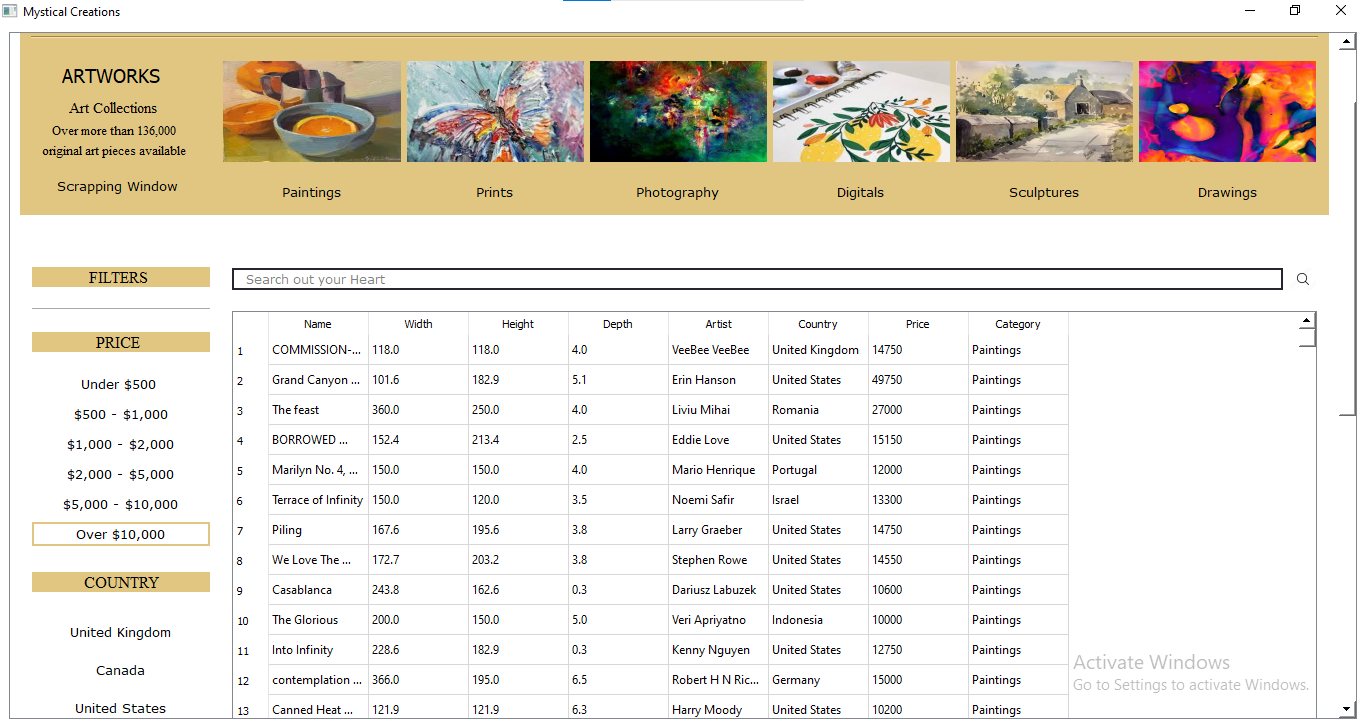
\includegraphics[width = 16cm, height = 9cm]{Price Filter.png}
	    \renewcommand{\thefigure}{3.11}
	    \caption{Data after Price filter is applied}
    \end{figure}
    \begin{figure}[ht!]
	    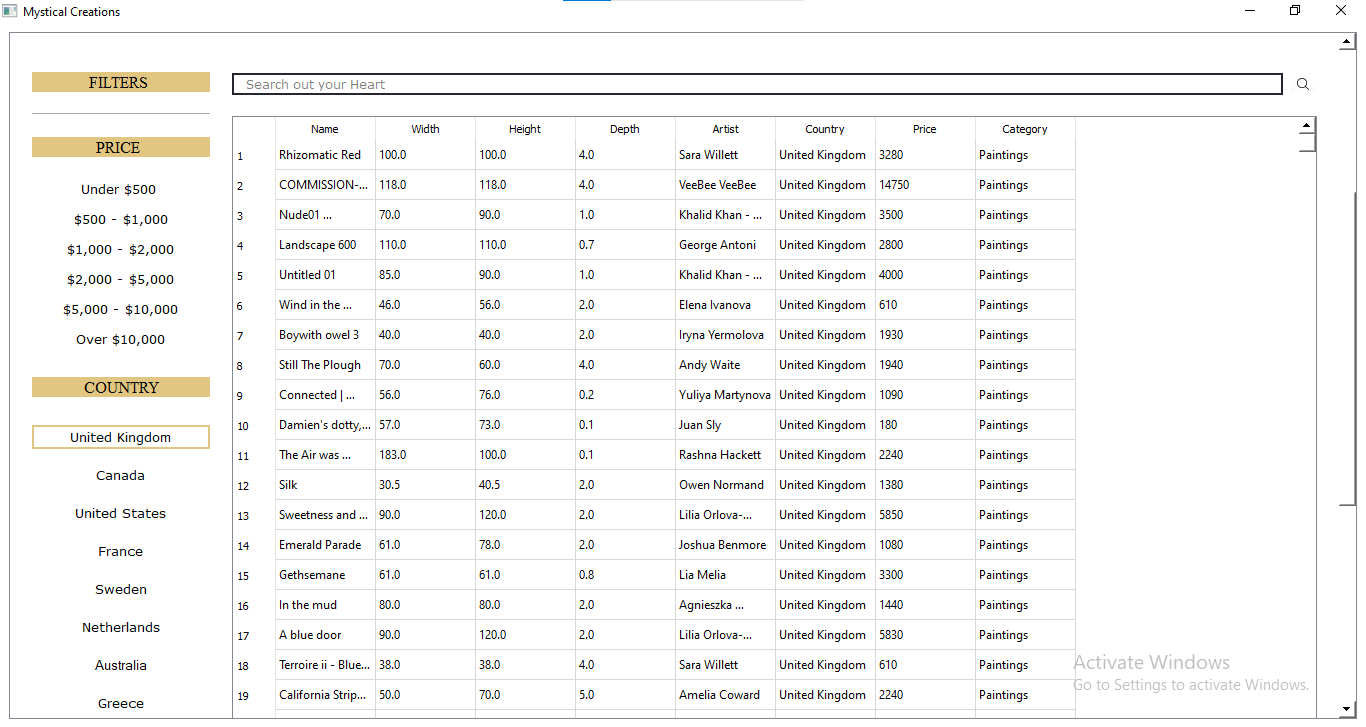
\includegraphics[width = 16cm, height = 9cm]{Country Filter.png}
	    \renewcommand{\thefigure}{3.12}
	    \caption{Data after Country filter is applied}
    \end{figure}
    
    \newpage
    \begin{figure}[ht!]
	    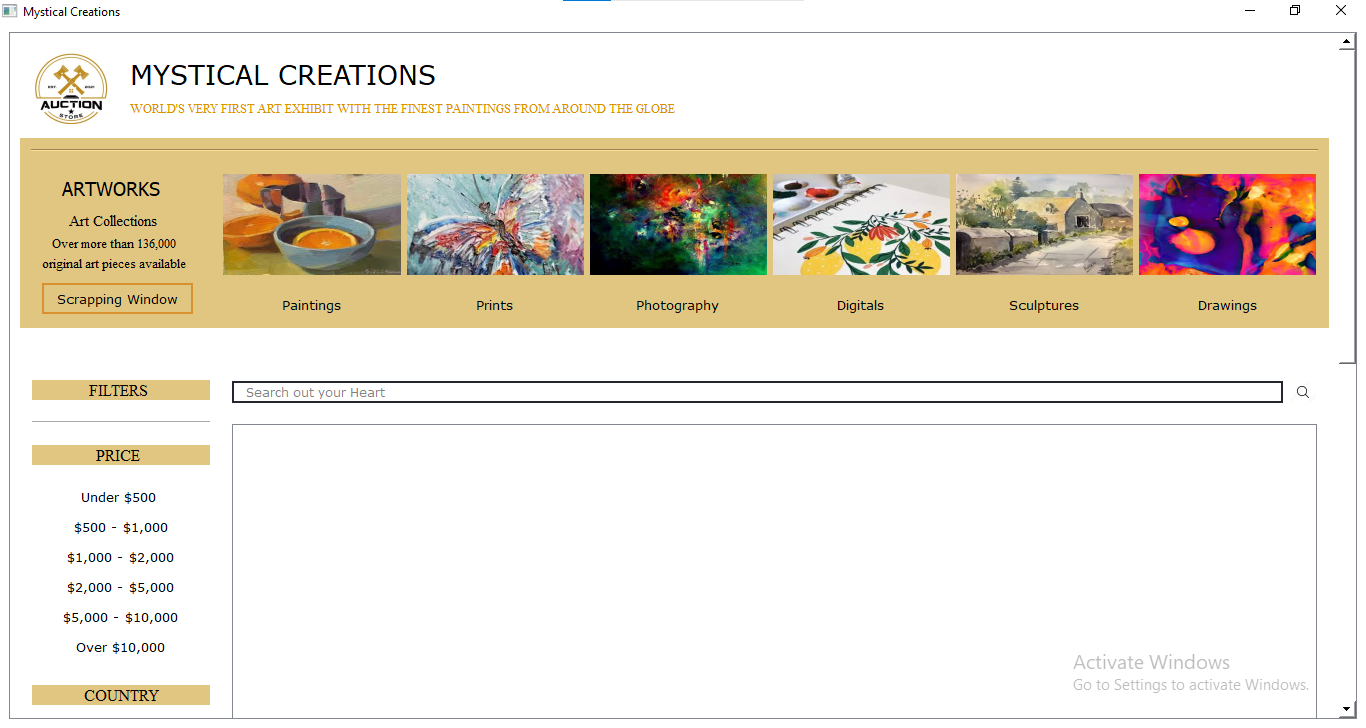
\includegraphics[width = 16cm, height = 9cm]{Scrapping Button.png}
	    \renewcommand{\thefigure}{3.13}
	    \caption{Scrapping Button}
    \end{figure}
    \begin{figure}[ht!]
	    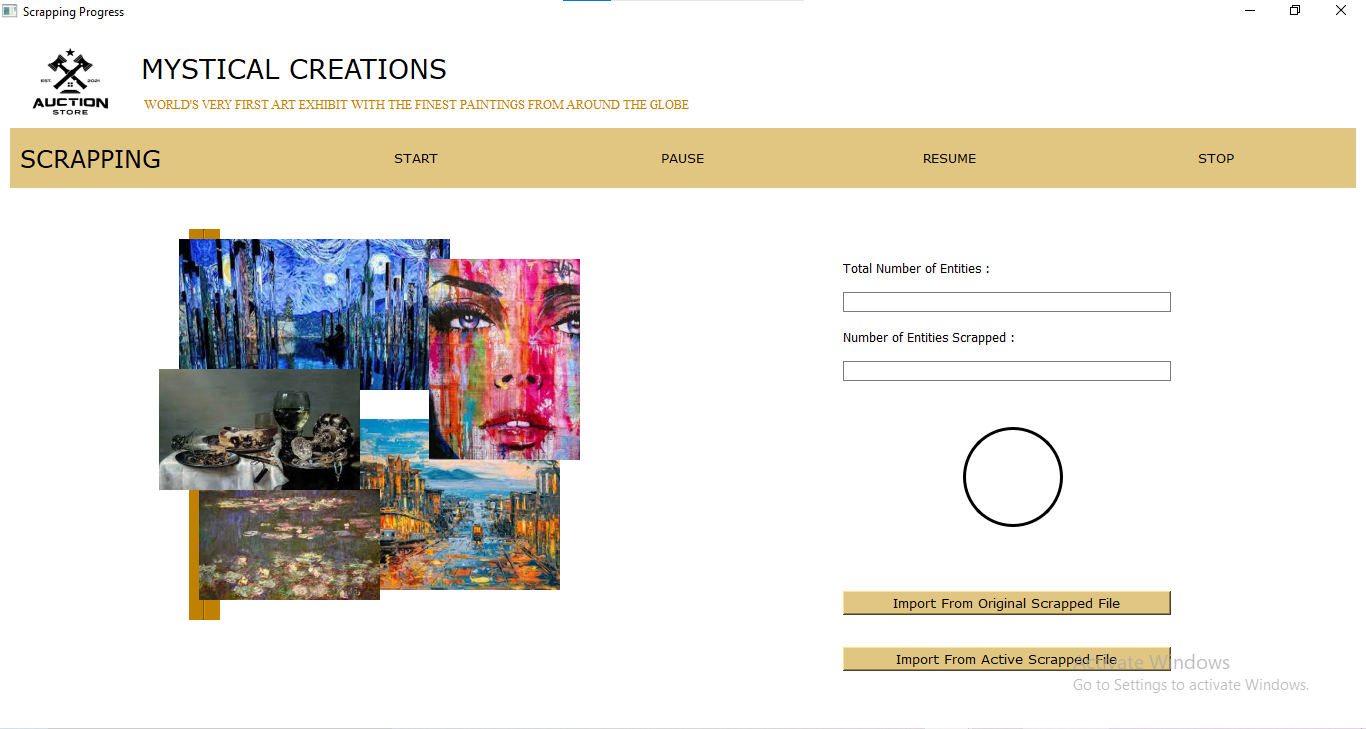
\includegraphics[width = 16cm, height = 9cm]{Scrapping Page.png}
	    \renewcommand{\thefigure}{3.14}
	    \caption{Layout of Scrapping Page}
    \end{figure}
    
    \newpage
    \subsection{Code}
    \begin{verbatim}
from dataclasses import dataclass
from tkinter import E
from PyQt5 import QtCore, QtGui, QtWidgets
from PyQt5.QtWidgets import QTableWidgetItem
from ScrappingPageResponsive_GUI import Ui_ScrappingWindow 
import pandas as pd
import sys
import numpy as np
import time
import csv
from csv import writer
from PyQt5.QtWidgets import *
from PyQt5.QtCore import *



class artPieces:

        def __init__(self, Name, Width, Height, Depth, Artist, Country,
        Price, Category):
                self.Name = Name
                self.Width = Width
                self.Height = Height
                self.Depth = Depth
                self.Artist = Artist
                self.Country = Country
                self.Price = Price 
                self.Category = Category


class Ui_MainWindow(object):

    dataList = []
    searchList = []

    def openScrappingWindow(self):
        self.window = QtWidgets.QMainWindow()
        self.ui = Ui_ScrappingWindow()
        self.ui.setupUi(self.window)
        self.window.show()


    def importData(self):
        self.dataList.clear()
        df = pd.read_csv(r'C:\Users\hassan\Documents\GitHub\cs261f22pid
        40\BackEndCode\Scrapping\DigitalsData.csv')

        df.fillna('', inplace = True)
        self.table.setRowCount(df.shape[0])
        self.table.setColumnCount(df.shape[1])
        self.table.setHorizontalHeaderLabels(df.columns)

        List = df.values.tolist()
        for i in range(0, len(List)):
                s = List[i][6].replace("$", "")
                s = s.replace(",", "")
                s = s.replace(".", "")
                x = int(s)
                self.dataList.append(artPieces(List[i][0], List[i][1],
                List[i][2], List[i][3], List[i][4], List[i][5], x,
                List[i][7]))


        self.reloadSortedListIntoTable()

    def reloadSortedListIntoTable(self):
        List = [[0 for i in range(8)] for j in
        range(len(self.dataList))]

        for i in range(0, len(self.dataList)):
                List[i][0] = self.dataList[i].Name
                List[i][1] = self.dataList[i].Width
                List[i][2] = self.dataList[i].Height
                List[i][3] = self.dataList[i].Depth
                List[i][4] = self.dataList[i].Artist
                List[i][5] = self.dataList[i].Country
                List[i][6] = self.dataList[i].Price
                List[i][7] = self.dataList[i].Category

        self.table.setRowCount(len(List))
        self.table.setColumnCount(len(List[0]))

        for row in range(len(List)):
                for col in range(len(List[0])):
                        tableItem =
                        QTableWidgetItem(str(List[row][col]))
                        self.table.setItem(row, col, tableItem)

    def reloadSearchList(self):
        
        List = [[0 for i in range(8)] for j in
        range(len(self.searchList))]

        for i in range(0, len(self.searchList)):
                List[i][0] = self.searchList[i].Name
                List[i][1] = self.searchList[i].Width
                List[i][2] = self.searchList[i].Height
                List[i][3] = self.searchList[i].Depth
                List[i][4] = self.searchList[i].Artist
                List[i][5] = self.searchList[i].Country
                List[i][6] = self.searchList[i].Price
                List[i][7] = self.searchList[i].Category

        self.table.setRowCount(len(List))
        self.table.setColumnCount(len(List[0]))

        for row in range(len(List)):
                for col in range(len(List[0])):
                        tableItem =
                        QTableWidgetItem(str(List[row][col]))
                        self.table.setItem(row, col, tableItem)


    def doSorting(self):
        algorithm = self.comboBoxSorting.currentText()
        column = self.comboBoxSortingColumn.currentText()

        if(algorithm == "Insertion Sort"): 
                start_time = time.time()
                self.InsertionSort(1, len(self.dataList), column)
                end_time = time.time()
                run_time = end_time - start_time
                self.reloadSortedListIntoTable()
                self.txtTime.setText(str(run_time))

        elif(algorithm == "Merge Sort"): 
                start_time = time.time()
                self.MergeSort(0, len(self.dataList) - 1, column)
                end_time = time.time()
                run_time = end_time - start_time
                self.reloadSortedListIntoTable()
                self.txtTime.setText(str(run_time))

        elif(algorithm == "Selection Sort"):
                start_time = time.time()
                self.SelectionSort(column)
                end_time = time.time()
                run_time = end_time - start_time
                self.reloadSortedListIntoTable()
                self.txtTime.setText(str(run_time))

        elif(algorithm == "Bubble Sort"):
                start_time = time.time()
                self.BubbleSort(column)
                end_time = time.time()
                run_time = end_time - start_time
                self.reloadSortedListIntoTable()
                self.txtTime.setText(str(run_time))

        elif(algorithm == "Heap Sort"):
                start_time = time.time()
                self.HeapSort(column)
                end_time = time.time()
                run_time = end_time - start_time
                self.reloadSortedListIntoTable()
                self.txtTime.setText(str(run_time))

        elif(algorithm == "Quick Sort"):
                start_time = time.time()
                self.QuickSort(0, len(self.dataList) - 1, column)
                end_time = time.time()
                run_time = end_time - start_time
                self.reloadSortedListIntoTable()
                self.txtTime.setText(str(run_time))

        elif(algorithm == "Genome Sort"):
                start_time = time.time()
                self.GenomeSort(column)
                end_time = time.time()
                run_time = end_time - start_time
                self.reloadSortedListIntoTable()
                self.txtTime.setText(str(run_time))

        elif(algorithm == "Cocktail Sort"):
                start_time = time.time()
                self.CocktailSort(column)
                end_time = time.time()
                run_time = end_time - start_time
                self.reloadSortedListIntoTable()
                self.txtTime.setText(str(run_time))

        elif(algorithm == "Shell Sort"): #setattr
                start_time = time.time()
                self.ShellSort(column)
                end_time = time.time()
                run_time = end_time - start_time
                self.reloadSortedListIntoTable()
                self.txtTime.setText(str(run_time))

        elif(algorithm == "Tim Sort"): #insertion and merge
                start_time = time.time()
                self.TimSort(column)
                end_time = time.time()
                run_time = end_time - start_time
                self.reloadSortedListIntoTable()
                self.txtTime.setText(str(run_time))
        
        elif(algorithm == "Counting Sort"):
                B = [0 for i in range(len(self.dataList))]
                max = getattr(self.dataList[0], column)

                for i in range (len(self.dataList)):
                        if getattr(self.dataList[i], column) > max:
                                max = getattr(self.dataList[i], column)
                                + 1 

                start_time = time.time()
                self.CountingSort(B, max, column)
                end_time = time.time()
                run_time = end_time - start_time
                self.reloadSortedListIntoTable()
                self.txtTime.setText(str(run_time))

        elif(algorithm == "Bucket Sort"):
                start_time = time.time()
                self.BucketSort(column)
                end_time = time.time()
                run_time = end_time - start_time
                self.reloadSortedListIntoTable()
                self.txtTime.setText(str(run_time))

        elif(algorithm == "Radix Sort"):
                start_time = time.time()
                self.RadixSort(column)
                end_time = time.time()
                run_time = end_time - start_time
                self.reloadSortedListIntoTable()
                self.txtTime.setText(str(run_time))

        elif(algorithm == "PigeonHole Sort"): 
                start_time = time.time()
                self.PigeonHoleSort(column)
                end_time = time.time()
                run_time = end_time - start_time
                self.reloadSortedListIntoTable()
                self.txtTime.setText(str(run_time))


    def Search(self):
        search = self.txtSearch.text()
        column = self.comboBoxSearchingColumn.currentText()
        searchAlgorithm = self.comboBoxSearching.currentText()

        if (searchAlgorithm == "Linear Search"):
                start_time = time.time()
                self.LinearSearch(search, column)
                end_time = time.time()
                run_time = end_time - start_time
                self.reloadSearchList()
                self.txtTime.setText(str(run_time))

        if (searchAlgorithm == "Starting Letter"):
                start_time = time.time()
                self.StartLetterSeacrh(search, column)
                end_time = time.time()
                run_time = end_time - start_time
                self.reloadSearchList()
                self.txtTime.setText(str(run_time))

        if (searchAlgorithm == "Middle Words"):
                start_time = time.time()
                self.MiddleWordsSearch(search, column)
                end_time = time.time()
                run_time = end_time - start_time
                self.reloadSearchList()
                self.txtTime.setText(str(run_time))
        

    def InsertionSort(self, p, r, column):
        i = 0
        key = 0

        for j in range(p, r):
                key = getattr(self.dataList[j], column)
                temp = self.dataList[j]
                i = j - 1
                
                while i >= 0 and getattr(self.dataList[i], column) >
                key:
                        temp = self.dataList[i + 1]
                        self.dataList[i + 1] = self.dataList[i]
                        i = i - 1 
                        self.dataList[i + 1] = temp


    def MergeSort(self, p, r, column):
        
        if p < r:
                q = int((p + r) / 2)
                self.MergeSort(p, q, column)
                self.MergeSort(q + 1, r, column)
                self.Merge(p, q, r, column)
    
    
    def Merge(self, p, q, r, column):
        n1 = q - p + 1
        n2 = r - q

        left_array = []
        right_array = []
        
        for i in range(n1):
                left_array.append(self.dataList[p + i])

        for j in range(n2):
                right_array.append(self.dataList[q + j + 1])

        x = artPieces(sys.maxsize, sys.maxsize, sys.maxsize,
        sys.maxsize, sys.maxsize, sys.maxsize, sys.maxsize, sys.maxsize)
        left_array.append(x)
        right_array.append(x)
        
        i = 0
        j = 0
        
        for k in range (p, r + 1):
                if getattr(left_array[i], column) <
                getattr(right_array[j], column):
                        self.dataList[k] = left_array[i]
                        i = i + 1
                else:
                        self.dataList[k] = right_array[j]
                        j = j + 1 


    def SelectionSort(self, column):
        start = 0
        end = len(self.dataList) - 1
        length = (end - start) + 1
        
        for i in range(length):
                min = i
                
                for j in range(i + 1, length):
                
                        if getattr(self.dataList[j], column) <
                        getattr(self.dataList[min], column):
                                min = j
                                
                (self.dataList[i], self.dataList[min]) =
                (self.dataList[min], self.dataList[i])


    def BubbleSort(self, column):
        start = 0
        end = len(self.dataList) - 1
    
        for i in range(start, end):
                
                for j in range(start, end):
                
                        if getattr(self.dataList[j], column) >
                        getattr(self.dataList[j + 1], column):
                                (self.dataList[j], self.dataList[j + 1])
                                = (self.dataList[j + 1], self.dataList[j])

    def maxHeapify(self, length, i, column):

        largest = i
        l = (2 * i) + 1
        r = (2 * i) + 2

        if l < length and getattr(self.dataList[l], column) >
        getattr(self.dataList[i], column):
                largest = l

        if r < length and getattr(self.dataList[r], column) >
        getattr(self.dataList[largest], column):
                largest = r

        if largest != i:
                (self.dataList[i], self.dataList[largest]) =
                (self.dataList[largest], self.dataList[i])
                self.maxHeapify(length, largest, column)

    def buildMaxHeapify(self, length, column):

        for i in range(length // 2, -1, -1):
                self.maxHeapify(length, i, column)

    def HeapSort(self, column):

        length = len(self.dataList)
        self.buildMaxHeapify(length, column)

        for i in range(length - 1, 0, -1):
                (self.dataList[i], self.dataList[0]) =
                (self.dataList[0], self.dataList[i])
                length = length - 1
                self.maxHeapify(i, 0, column)


    def partition(self, p, r, column):
        x = getattr(self.dataList[r], column)
        i = p - 1

        for j in range(p, r):
                if getattr(self.dataList[j], column) <= x:
                        i = i + 1
                        (self.dataList[i], self.dataList[j]) =
                        (self.dataList[j], self.dataList[i])
        
        (self.dataList[i + 1], self.dataList[r]) = (self.dataList[r],
        self.dataList[i + 1])
        return i + 1


    def QuickSort(self, p, r, column):
        if p < r:
                q = self.partition(p, r, column)
                self.QuickSort(p, q - 1, column)
                self.QuickSort(q + 1, r, column)


    def GenomeSort(self, column):
        length = len(self.dataList)
        idx = 0 

        while idx < length:

                if idx == 0 or getattr(self.dataList[idx], column) >=
                getattr(self.dataList[idx - 1], column):
                        idx = idx + 1

                else:
                        (self.dataList[idx], self.dataList[idx - 1]) =
                        (self.dataList[idx - 1], self.dataList[idx])
                        idx = idx - 1


    def CocktailSort(self, column):
        length = len(self.dataList)

        for i in range(length - 1, 0, -1):

                for j in range(i):
                        if getattr(self.dataList[j], column) >
                        getattr(self.dataList[j + 1], column):
                                (self.dataList[j], self.dataList[j + 1])
                                = (self.dataList[j + 1], self.dataList[j])

                for j in range(i, 0, -1):
                        if getattr(self.dataList[j], column) <
                        getattr(self.dataList[j - 1], column):
                                (self.dataList[j], self.dataList[j - 1])
                                = (self.dataList[j - 1], self.dataList[j]) 

    
    def ShellSort(self, column):

        gap = len(self.dataList)//2
     
        while gap>0:
                j = gap
                
                while j < len(self.dataList):
                        i = j - gap 
                        
                        while i >= 0:
                                
                                if getattr(self.dataList[i + gap],
                                column) > getattr(self.dataList[i],
                                column):
                                        break
                                else:
                                        self.dataList[i+gap],
                                        self.dataList[i] =
                                        self.dataList[i],
                                        self.dataList[i+gap]
                
                                i = i - gap 

                        j = j + 1
                        
                gap = gap // 2


    def TimSort(self, column):
        length = len(self.dataList)
        minRun = 32

        for p in range(0, length, minRun):
                r = min(p + minRun - 1, length -1)
                self.InsertionSort(p, r, column)

        size = minRun
        while size < length:
                for p in range(0, length, 2 * size):
                        q = min(length - 1, p + size - 1)
                        r = min((p + 2 * size - 1), (length - 1))

                        if q < r:
                                self.Merge(p, q, r, column)        

                size = 2 * size

                
    def CountingSort(self, B, max, column):

        C = []
        Result = []

        for i in range (max):
                C.append(0)

        for j in range (len(self.dataList)):
                C[getattr(self.dataList[j], column)] =
                C[getattr(self.dataList[j], column)] + 1

        for i in range (1, max):
                C[i] = C[i] + C[i - 1]

        for j in range (len(self.dataList), 0 , -1):
                B[(C[getattr(self.dataList[j-1], column)]) - 1] =
                self.dataList[j - 1]      
                C[getattr(self.dataList[j - 1], column)] =
                C[getattr(self.dataList[j - 1], column)] - 1

        for i in range (len(self.dataList)):
                self.dataList[i] = B[i]


    def BucketInsertionSort(self, array):
        i = 0
        key = 0

        for j in range(1, len(array)):
                key = array[j]
                i = j - 1
        
                while i >= 0 and array[i] > key:
                        array[i+1] = array[i]
                        i = i - 1 
                        array[i + 1] = key


    def BucketSort(self, column):
        B = []
        n = len(column)

        for i in range (n):
                B.append([])

        for i in range (n):
                B[int(n * getattr(self.dataList[i],
                column))].append(self.dataList[i])

        for i in range (n):
                B[i] = self.BucketInsertionSort(B[i])

        B = np.concatenate(B)
        return B 


    def RadixCountingSort(self, B, n, column):
        C = [0] * 10

        for j in range (len(self.dataList)):
                temp = getattr(self.dataList[j], column) // n
                C[temp % 10] = C[temp % 10] + 1

        for i in range (1, 10):
                C[i] = C[i] + C[i - 1]

        i = len(self.dataList) - 1
        while (i >= 0):
                temp = getattr(self.dataList[i], column) // n 
                B[C[temp % 10] - 1] = self.dataList[i]
                C[temp % 10] = C[temp % 10] - 1
                i = i - 1

        for i in range (len(self.dataList)):
                self.dataList[i] = B[i]

    def RadixSort(self, column):
        d = -1

        for i in range(0, len(self.dataList)):
                if d > getattr(self.dataList[i], column):
                        d = getattr(self.dataList[i], column)

        B = [0 for i in range(len(self.dataList))]
        n = 1
        while (d // n > 0):
                self.dataList = self.RadixCountingSort(B, n, column)
                n = n * 10


    def PigeonHoleSort(self, column):
        Smallest = 9999999999
        Largest = -1

        for i in range(0, len(self.dataList)):
                if Smallest > getattr(self.dataList[i], column):
                        Smallest = getattr(self.dataList[i], column)

        for i in range(0, len(self.dataList)):
                if Largest < getattr(self.dataList[i], column):
                        Largest = getattr(self.dataList[i], column)

        
        NumberOfHoles = Largest - Smallest + 1
        Holes = []

        for i in range (NumberOfHoles):
                Holes.append(0)

        for j in self.dataList:
                Holes[j - Smallest] = Holes[j - Smallest] + 1

        self.dataList.clear()
        for x in range (NumberOfHoles):
                while (Holes[x] > 0):
                        Holes[x] = Holes[x] - 1
                        self.dataList.append(x + Smallest)


    def LinearSearch(self, search, column):

        if column == "Width" or column == "Height" or column == "Depth":
                search = float(search)

        elif column == "Price":
                search = int(search)

        for i in range(0, len(self.dataList)):
                        if getattr(self.dataList[i], column) == search:
                                self.searchList.append(self.dataList[i])

    def StartLetterSeacrh(self, search, column):
        length = len(self.dataList)

        for i in range(0, length):
                if column == "Width" or column == "Height" or column ==
                "Depth" or column == "Price":
                        attribute = getattr(self.dataList[i], column)
                        attribute = str(attribute)

                else:
                        attribute = getattr(self.dataList[i], column)

                if attribute[0] == search:
                        self.searchList.append(self.dataList[i])

    def MiddleWordsSearch(self, search, column):
        for i in range(0, len(self.dataList)):
                
                attribute = getattr(self.dataList[i], column)
                wordList = attribute.split()

                for j in range(0, len(wordList)):
                        if wordList[j] == search:
                                self.searchList.append(self.dataList[i])

    def SearchPaintingsBtn(self):
                for i in range(0, len(self.dataList)):
                        if self.dataList[i].Category == "Paintings":
                                self.searchList.append(self.dataList[i])
                
                self.reloadSearchList()


    def SearchPrintsBtn(self):
                for i in range(0, len(self.dataList)):
                        if self.dataList[i].Category == "Prints":
                                self.searchList.append(self.dataList[i])
                
                self.reloadSearchList()


    def SearchDigitalsBtn(self):
                for i in range(0, len(self.dataList)):
                        if self.dataList[i].Category == "Digitals":
                                self.searchList.append(self.dataList[i])
                
                self.reloadSearchList()


    def SearchSculpturesBtn(self):
                for i in range(0, len(self.dataList)):
                        if self.dataList[i].Category == "Sculptures":
                                self.searchList.append(self.dataList[i])
                
                self.reloadSearchList()


    def SearchDrawingsBtn(self):
                for i in range(0, len(self.dataList)):
                        if self.dataList[i].Category == "Drawings":
                                self.searchList.append(self.dataList[i])
                
                self.reloadSearchList()


    def SearchPhotographyBtn(self):
                for i in range(0, len(self.dataList)):
                        if self.dataList[i].Category == "Photography":
                                self.searchList.append(self.dataList[i])
                
                self.reloadSearchList()

    def SearchUKBtn(self):
                for i in range(0, len(self.dataList)):
                        if self.dataList[i].Country == "United Kingdom":
                                self.searchList.append(self.dataList[i])
                
                self.reloadSearchList()

    def SearchCanadaBtn(self):
                for i in range(0, len(self.dataList)):
                        if self.dataList[i].Country == "Canada":
                                self.searchList.append(self.dataList[i])
                
                self.reloadSearchList()

    def SearchUSBtn(self):
                for i in range(0, len(self.dataList)):
                        if self.dataList[i].Country == "United States":
                                self.searchList.append(self.dataList[i])
                
                self.reloadSearchList()

    def SearchFranceBtn(self):
                for i in range(0, len(self.dataList)):
                        if self.dataList[i].Country == "France":
                                self.searchList.append(self.dataList[i])
                
                self.reloadSearchList()

    def SearchSwedenBtn(self):
                for i in range(0, len(self.dataList)):
                        if self.dataList[i].Country == "Sweden":
                                self.searchList.append(self.dataList[i])
                
                self.reloadSearchList()

    def SearchNetherlandsBtn(self):
                for i in range(0, len(self.dataList)):
                        if self.dataList[i].Country == "Netherlands":
                                self.searchList.append(self.dataList[i])
                
                self.reloadSearchList()

    def SearchAustraliaBtn(self):
                for i in range(0, len(self.dataList)):
                        if self.dataList[i].Country == "Australia":
                                self.searchList.append(self.dataList[i])
                
                self.reloadSearchList()

    def SearchGreeceBtn(self):
                for i in range(0, len(self.dataList)):
                        if self.dataList[i].Country == "Greece":
                                self.searchList.append(self.dataList[i])
                
                self.reloadSearchList()

    def SearchSwitzerlandBtn(self):
                for i in range(0, len(self.dataList)):
                        if self.dataList[i].Country == "Switzerland":
                                self.searchList.append(self.dataList[i])
                
                self.reloadSearchList()

    def SearchSpainBtn(self):
                for i in range(0, len(self.dataList)):
                        if self.dataList[i].Country == "Spain":
                                self.searchList.append(self.dataList[i])
                
                self.reloadSearchList()

    def SearchMexicoBtn(self):
                for i in range(0, len(self.dataList)):
                        if self.dataList[i].Country == "Mexico":
                                self.searchList.append(self.dataList[i])
                
                self.reloadSearchList()

    def SearchPakistanBtn(self):
                for i in range(0, len(self.dataList)):
                        if self.dataList[i].Country == "Pakistan":
                                self.searchList.append(self.dataList[i])
                
                self.reloadSearchList()

    def SearchSABtn(self):
                for i in range(0, len(self.dataList)):
                        if self.dataList[i].Country == "South Africa":
                                self.searchList.append(self.dataList[i])
                
                self.reloadSearchList()

    def SearchItalyBtn(self):
                for i in range(0, len(self.dataList)):
                        if self.dataList[i].Country == "Italy":
                                self.searchList.append(self.dataList[i])
                
                self.reloadSearchList()

    def SearchNZBtn(self):
                for i in range(0, len(self.dataList)):
                        if self.dataList[i].Country == "New Zealand":
                                self.searchList.append(self.dataList[i])
                
                self.reloadSearchList()

    def SearchGermanyBtn(self):
                for i in range(0, len(self.dataList)):
                        if self.dataList[i].Country == "Germany":
                                self.searchList.append(self.dataList[i])
                
                self.reloadSearchList()

    def SearchIndiaBtn(self):
                for i in range(0, len(self.dataList)):
                        if self.dataList[i].Country == "India":
                                self.searchList.append(self.dataList[i])
                
                self.reloadSearchList()

    def SearchChinaBtn(self):
                for i in range(0, len(self.dataList)):
                        if self.dataList[i].Country == "China":
                                self.searchList.append(self.dataList[i])
                
                self.reloadSearchList()

    def SearchUnder500Btn(self):
                for i in range(0, len(self.dataList)):
                        if self.dataList[i].Price >= 0 and
                        self.dataList[i].Price < 500:
                                self.searchList.append(self.dataList[i])
                
                self.reloadSearchList()

    def Search500to1000Btn(self):
                for i in range(0, len(self.dataList)):
                        if self.dataList[i].Price >= 500 and
                        self.dataList[i].Price < 1000:
                                self.searchList.append(self.dataList[i])
                
                self.reloadSearchList()

    def Search1000to2000Btn(self):
                for i in range(0, len(self.dataList)):
                        if self.dataList[i].Price >= 1000 and
                        self.dataList[i].Price < 2000:
                                self.searchList.append(self.dataList[i])
                
                self.reloadSearchList()

    def Search2000to5000Btn(self):
                for i in range(0, len(self.dataList)):
                        if self.dataList[i].Price >= 2000 and
                        self.dataList[i].Price < 5000:
                                self.searchList.append(self.dataList[i])
                
                self.reloadSearchList()

    def Search5000to10000Btn(self):
                for i in range(0, len(self.dataList)):
                        if self.dataList[i].Price >= 5000 and
                        self.dataList[i].Price < 10000:
                                self.searchList.append(self.dataList[i])
                
                self.reloadSearchList()

    def SearchOver10000Btn(self):
                for i in range(0, len(self.dataList)):
                        if self.dataList[i].Price >= 10000:
                                self.searchList.append(self.dataList[i])
                
                self.reloadSearchList()

    def Export(self):
        info = [0] * 7

        List = [[0 for i in range(8)] for j in range(len(self.dataList))]

        for i in range(0, len(self.dataList)):
                List[i][0] = self.dataList[i].Name
                List[i][1] = self.dataList[i].Width
                List[i][2] = self.dataList[i].Height
                List[i][3] = self.dataList[i].Depth
                List[i][4] = self.dataList[i].Artist
                List[i][5] = self.dataList[i].Country
                List[i][6] = self.dataList[i].Price
                List[i][7] = self.dataList[i].Category

        with open('ExportFile.csv', "w", encoding='utf8', newline='') as
        f:
    
                thewriter =  writer(f)
                header = ['Name', 'Width', 'Height', 'Depth', 'Painter',
                'Country','Price', 'Category']
                thewriter.writerow(header)

                for row in range(len(List)):
                        for col in range(len(List[0])):
                                info[col] = QTableWidgetItem(str(List[row][col]))

                        thewriter.writerow(info)
                        info.clear()


        self.dataList.clear()
        self.table.clear()
        self.table.setRowCount(0)
        self.table.setColumnCount(0)

        

    def setupUi(self, MainWindow):
        MainWindow.setObjectName("MainWindow")
        MainWindow.resize(1200, 850)
        MainWindow.setMinimumSize(QtCore.QSize(550, 100))
        MainWindow.setStyleSheet("background-color: rgb(255, 255, 255);")
        self.centralwidget = QtWidgets.QWidget(MainWindow)
        self.centralwidget.setObjectName("centralwidget")
        self.verticalLayout = QtWidgets.QVBoxLayout(self.centralwidget)
        self.verticalLayout.setObjectName("verticalLayout")
        self.scrollArea = QtWidgets.QScrollArea(self.centralwidget)
        self.scrollArea.setWidgetResizable(True)
        self.scrollArea.setObjectName("scrollArea")
        self.scrollAreaWidgetContents = QtWidgets.QWidget()
        self.scrollAreaWidgetContents.setGeometry(QtCore.QRect(0, -215,
        826, 1412))
        self.scrollAreaWidgetContents.setObjectName("scrollAreaWidget
        Contents")
        self.verticalLayout_2 =
        QtWidgets.QVBoxLayout(self.scrollAreaWidgetContents)
        self.verticalLayout_2.setObjectName("verticalLayout_2")
        self.frame = QtWidgets.QFrame(self.scrollAreaWidgetContents)
        self.frame.setMinimumSize(QtCore.QSize(0, 1400))
        self.frame.setFrameShape(QtWidgets.QFrame.StyledPanel)
        self.frame.setFrameShadow(QtWidgets.QFrame.Raised)
        self.frame.setObjectName("frame")
        self.verticalLayout_3 = QtWidgets.QVBoxLayout(self.frame)
        self.verticalLayout_3.setContentsMargins(0, 0, 0, 0)
        self.verticalLayout_3.setSpacing(0)
        self.verticalLayout_3.setObjectName("verticalLayout_3")
        self.frame_2 = QtWidgets.QFrame(self.frame)
        self.frame_2.setMinimumSize(QtCore.QSize(0, 95))
        self.frame_2.setMaximumSize(QtCore.QSize(16777215, 95))
        self.frame_2.setFrameShape(QtWidgets.QFrame.StyledPanel)
        self.frame_2.setFrameShadow(QtWidgets.QFrame.Raised)
        self.frame_2.setObjectName("frame_2")
        self.label_2 = QtWidgets.QLabel(self.frame_2)
        self.label_2.setGeometry(QtCore.QRect(10, 10, 81, 71))
        self.label_2.setStyleSheet("background-image:url(:/resource/
        graphics/Auction.jpg)")
        self.label_2.setText("")
        self.label_2.setPixmap(QtGui.QPixmap(":/resource/graphics/
        Auction.jpg"))
        self.label_2.setScaledContents(True)
        self.label_2.setObjectName("label_2")
        self.label = QtWidgets.QLabel(self.frame_2)
        self.label.setGeometry(QtCore.QRect(110, 10, 441, 41))
        self.label.setStyleSheet("font: 20pt \"MS Reference Sans
        Serif\";")
        self.label.setObjectName("label")
        self.label_3 = QtWidgets.QLabel(self.frame_2)
        self.label_3.setGeometry(QtCore.QRect(110, 50, 671, 31))
        font = QtGui.QFont()
        font.setFamily("Times New Roman")
        font.setPointSize(10)
        font.setBold(False)
        font.setItalic(False)
        font.setWeight(50)
        self.label_3.setFont(font)
        self.label_3.setStyleSheet("font: 10pt \"Times New Roman\";\n"
"color:rgb(217, 145, 0)")
        self.label_3.setScaledContents(False)
        self.label_3.setObjectName("label_3")
        self.pushButton = QtWidgets.QPushButton(self.frame_2)
        self.pushButton.setGeometry(QtCore.QRect(60, 60, 31, 31))
        self.pushButton.setStyleSheet("background-image:url(:/newPrefix
        /Downloads/P19.png)")
        self.pushButton.setText("")
        icon = QtGui.QIcon()
        icon.addPixmap(QtGui.QPixmap(":/newPrefix/Downloads/P19.png"),
        QtGui.QIcon.Normal, QtGui.QIcon.Off)
        self.pushButton.setIcon(icon)
        self.pushButton.setFlat(True)
        self.pushButton.setObjectName("pushButton")
        self.verticalLayout_3.addWidget(self.frame_2)
        self.frame_3 = QtWidgets.QFrame(self.frame)
        self.frame_3.setMaximumSize(QtCore.QSize(16777215, 190))
        self.frame_3.setStyleSheet("background-color:rgb(225, 198,
        129)")
        self.frame_3.setFrameShape(QtWidgets.QFrame.StyledPanel)
        self.frame_3.setFrameShadow(QtWidgets.QFrame.Raised)
        self.frame_3.setObjectName("frame_3")
        self.verticalLayout_4 = QtWidgets.QVBoxLayout(self.frame_3)
        self.verticalLayout_4.setContentsMargins(0, 0, 0, 0)
        self.verticalLayout_4.setSpacing(0)
        self.verticalLayout_4.setObjectName("verticalLayout_4")
        self.frame_4 = QtWidgets.QFrame(self.frame_3)
        self.frame_4.setMinimumSize(QtCore.QSize(0, 0))
        self.frame_4.setMaximumSize(QtCore.QSize(16777215, 25))
        self.frame_4.setFrameShape(QtWidgets.QFrame.StyledPanel)
        self.frame_4.setFrameShadow(QtWidgets.QFrame.Raised)
        self.frame_4.setObjectName("frame_4")
        self.verticalLayout_6 = QtWidgets.QVBoxLayout(self.frame_4)
        self.verticalLayout_6.setObjectName("verticalLayout_6")
        self.line = QtWidgets.QFrame(self.frame_4)
        self.line.setMinimumSize(QtCore.QSize(0, 0))
        self.line.setStyleSheet("")
        self.line.setFrameShape(QtWidgets.QFrame.HLine)
        self.line.setFrameShadow(QtWidgets.QFrame.Sunken)
        self.line.setObjectName("line")
        self.verticalLayout_6.addWidget(self.line)
        self.verticalLayout_4.addWidget(self.frame_4)
        self.frame_6 = QtWidgets.QFrame(self.frame_3)
        self.frame_6.setFrameShape(QtWidgets.QFrame.StyledPanel)
        self.frame_6.setFrameShadow(QtWidgets.QFrame.Raised)
        self.frame_6.setObjectName("frame_6")
        self.horizontalLayout = QtWidgets.QHBoxLayout(self.frame_6)
        self.horizontalLayout.setContentsMargins(0, 0, 0, 0)
        self.horizontalLayout.setSpacing(0)
        self.horizontalLayout.setObjectName("horizontalLayout")
        self.frame_7 = QtWidgets.QFrame(self.frame_6)
        self.frame_7.setMinimumSize(QtCore.QSize(190, 0))
        self.frame_7.setMaximumSize(QtCore.QSize(175, 16777215))
        self.frame_7.setFrameShape(QtWidgets.QFrame.StyledPanel)
        self.frame_7.setFrameShadow(QtWidgets.QFrame.Raised)
        self.frame_7.setObjectName("frame_7")
        self.label_4 = QtWidgets.QLabel(self.frame_7)
        self.label_4.setGeometry(QtCore.QRect(40, 10, 141, 31))
        self.label_4.setStyleSheet("font: 14pt \"MS Shell Dlg 2\";")
        self.label_4.setObjectName("label_4")
        self.label_5 = QtWidgets.QLabel(self.frame_7)
        self.label_5.setGeometry(QtCore.QRect(40, 50, 141, 16))
        self.label_5.setStyleSheet("font: 11pt \"Times New Roman\";")
        self.label_5.setObjectName("label_5")
        self.label_13 = QtWidgets.QLabel(self.frame_7)
        self.label_13.setGeometry(QtCore.QRect(30, 70, 161, 21))
        self.label_13.setStyleSheet("font: 10pt \"Times New Roman\";")
        self.label_13.setObjectName("label_13")
        self.label_15 = QtWidgets.QLabel(self.frame_7)
        self.label_15.setGeometry(QtCore.QRect(20, 90, 171, 21))
        self.label_15.setStyleSheet("font: 10pt \"Times New Roman\";")
        self.label_15.setObjectName("label_15")
        self.btnScrappingWindow = QtWidgets.QPushButton(self.frame_7,
        clicked = lambda: self.openScrappingWindow())
        self.btnScrappingWindow.setGeometry(QtCore.QRect(20, 120, 151,
        31))
        self.btnScrappingWindow.setMinimumSize(QtCore.QSize(80, 20))
        font = QtGui.QFont()
        font.setFamily("MS Reference Sans Serif")
        font.setPointSize(10)
        self.btnScrappingWindow.setFont(font)
        self.btnScrappingWindow.setStyleSheet("QPushButton:hover{\n"
"border: 2px solid rgb(217, 145, 48);\n"
"}")
        self.btnScrappingWindow.setAutoDefault(False)
        self.btnScrappingWindow.setDefault(False)
        self.btnScrappingWindow.setFlat(True)
        self.btnScrappingWindow.setObjectName("btnScrappingWindow")
        self.horizontalLayout.addWidget(self.frame_7)
        self.frame_8 = QtWidgets.QFrame(self.frame_6)
        self.frame_8.setFrameShape(QtWidgets.QFrame.StyledPanel)
        self.frame_8.setFrameShadow(QtWidgets.QFrame.Raised)
        self.frame_8.setObjectName("frame_8")
        self.verticalLayout_5 = QtWidgets.QVBoxLayout(self.frame_8)
        self.verticalLayout_5.setContentsMargins(0, 0, 0, 0)
        self.verticalLayout_5.setSpacing(0)
        self.verticalLayout_5.setObjectName("verticalLayout_5")
        self.frame_9 = QtWidgets.QFrame(self.frame_8)
        self.frame_9.setMinimumSize(QtCore.QSize(550, 100))
        self.frame_9.setFrameShape(QtWidgets.QFrame.StyledPanel)
        self.frame_9.setFrameShadow(QtWidgets.QFrame.Raised)
        self.frame_9.setObjectName("frame_9")
        self.horizontalLayout_2 = QtWidgets.QHBoxLayout(self.frame_9)
        self.horizontalLayout_2.setObjectName("horizontalLayout_2")
        self.label_6 = QtWidgets.QLabel(self.frame_9)
        self.label_6.setStyleSheet("background-image:url(:/resource/
        graphics/P12.jpg)")
        self.label_6.setText("")
        self.label_6.setPixmap(QtGui.QPixmap(":/resource/graphics/P12
        .jpg"))
        self.label_6.setScaledContents(True)
        self.label_6.setObjectName("label_6")
        self.horizontalLayout_2.addWidget(self.label_6)
        self.label_7 = QtWidgets.QLabel(self.frame_9)
        self.label_7.setStyleSheet("background-image:url(:/resource/
        graphics/P5.jpg)")
        self.label_7.setText("")
        self.label_7.setPixmap(QtGui.QPixmap(":/resource/graphics/
        P5.jpg"))
        self.label_7.setScaledContents(True)
        self.label_7.setObjectName("label_7")
        self.horizontalLayout_2.addWidget(self.label_7)
        self.label_8 = QtWidgets.QLabel(self.frame_9)
        self.label_8.setStyleSheet("background-image:url(:/resource/
        graphics/P41.jpg)")
        self.label_8.setText("")
        self.label_8.setPixmap(QtGui.QPixmap(":/resource/graphics/
        P41.jpg"))
        self.label_8.setScaledContents(True)
        self.label_8.setObjectName("label_8")
        self.horizontalLayout_2.addWidget(self.label_8)
        self.label_9 = QtWidgets.QLabel(self.frame_9)
        self.label_9.setStyleSheet("background-image:url(:/resource/
        graphics/P8.jpg)")
        self.label_9.setText("")
        self.label_9.setPixmap(QtGui.QPixmap(":/resource/graphics/
        P8.jpg"))
        self.label_9.setScaledContents(True)
        self.label_9.setObjectName("label_9")
        self.horizontalLayout_2.addWidget(self.label_9)
        self.label_10 = QtWidgets.QLabel(self.frame_9)
        self.label_10.setStyleSheet("background-image:url(:/resource/
        graphics/P14.jpg)")
        self.label_10.setText("")
        self.label_10.setPixmap(QtGui.QPixmap(":/resource/graphics/
        P14.jpg"))
        self.label_10.setScaledContents(True)
        self.label_10.setObjectName("label_10")
        self.horizontalLayout_2.addWidget(self.label_10)
        self.label_11 = QtWidgets.QLabel(self.frame_9)
        self.label_11.setStyleSheet("background-image:url(:/resource/
        graphics/P11.jpg)")
        self.label_11.setText("")
        self.label_11.setPixmap(QtGui.QPixmap(":/resource/graphics/
        P11.jpg"))
        self.label_11.setScaledContents(True)
        self.label_11.setObjectName("label_11")
        self.horizontalLayout_2.addWidget(self.label_11)
        self.verticalLayout_5.addWidget(self.frame_9)
        self.frame_10 = QtWidgets.QFrame(self.frame_8)
        self.frame_10.setMinimumSize(QtCore.QSize(0, 40))
        self.frame_10.setMaximumSize(QtCore.QSize(16777215, 40))
        self.frame_10.setFrameShape(QtWidgets.QFrame.StyledPanel)
        self.frame_10.setFrameShadow(QtWidgets.QFrame.Raised)
        self.frame_10.setObjectName("frame_10")
        self.horizontalLayout_3 = QtWidgets.QHBoxLayout(self.frame_10)
        self.horizontalLayout_3.setObjectName("horizontalLayout_3")
        self.btnPaintings = QtWidgets.QPushButton(self.frame_10, clicked
        = lambda: self.SearchPaintingsBtn())
        self.btnPaintings.setMinimumSize(QtCore.QSize(80, 20))
        font = QtGui.QFont()
        font.setFamily("MS Reference Sans Serif")
        font.setPointSize(10)
        self.btnPaintings.setFont(font)
        self.btnPaintings.setStyleSheet("QPushButton:hover{\n"
"border: 2px solid rgb(217, 145, 48);\n"
"}")
        self.btnPaintings.setFlat(True)
        self.btnPaintings.setObjectName("btnPaintings")
        self.horizontalLayout_3.addWidget(self.btnPaintings)
        self.btnPrints = QtWidgets.QPushButton(self.frame_10, clicked 
        = lambda: self.SearchPrintsBtn())
        self.btnPrints.setMinimumSize(QtCore.QSize(80, 20))
        font = QtGui.QFont()
        font.setFamily("MS Reference Sans Serif")
        font.setPointSize(10)
        self.btnPrints.setFont(font)
        self.btnPrints.setStyleSheet("QPushButton:hover{\n"
"border: 2px solid rgb(217, 145, 48);\n"
"}")
        self.btnPrints.setFlat(True)
        self.btnPrints.setObjectName("btnPrints")
        self.horizontalLayout_3.addWidget(self.btnPrints)
        self.btnPhotography = QtWidgets.QPushButton(self.frame_10,
        clicked = lambda: self.SearchPhotographyBtn())
        self.btnPhotography.setMinimumSize(QtCore.QSize(80, 20))
        font = QtGui.QFont()
        font.setFamily("MS Reference Sans Serif")
        font.setPointSize(10)
        self.btnPhotography.setFont(font)
        self.btnPhotography.setStyleSheet("QPushButton:hover{\n"
"border: 2px solid rgb(217, 145, 48);\n"
"}")
        self.btnPhotography.setFlat(True)
        self.btnPhotography.setObjectName("btnPhotography")
        self.horizontalLayout_3.addWidget(self.btnPhotography)
        self.btnDigitals = QtWidgets.QPushButton(self.frame_10, 
        clicked = lambda: self.SearchDigitalsBtn())
        self.btnDigitals.setMinimumSize(QtCore.QSize(80, 20))
        font = QtGui.QFont()
        font.setFamily("MS Reference Sans Serif")
        font.setPointSize(10)
        self.btnDigitals.setFont(font)
        self.btnDigitals.setStyleSheet("QPushButton:hover{\n"
"border: 2px solid rgb(217, 145, 48);\n"
"}")
        self.btnDigitals.setFlat(True)
        self.btnDigitals.setObjectName("btnDigitals")
        self.horizontalLayout_3.addWidget(self.btnDigitals)
        self.btnSculptures = QtWidgets.QPushButton(self.frame_10,
        clicked = lambda: self.SearchSculpturesBtn())
        self.btnSculptures.setMinimumSize(QtCore.QSize(80, 20))
        font = QtGui.QFont()
        font.setFamily("MS Reference Sans Serif")
        font.setPointSize(10)
        self.btnSculptures.setFont(font)
        self.btnSculptures.setStyleSheet("QPushButton:hover{\n"
"border: 2px solid rgb(217, 145, 48);\n"
"}")
        self.btnSculptures.setFlat(True)
        self.btnSculptures.setObjectName("btnSculptures")
        self.horizontalLayout_3.addWidget(self.btnSculptures)
        self.btnDrawings = QtWidgets.QPushButton(self.frame_10, 
        clicked = lambda: self.SearchDrawingsBtn())
        self.btnDrawings.setMinimumSize(QtCore.QSize(80, 20))
        font = QtGui.QFont()
        font.setFamily("MS Reference Sans Serif")
        font.setPointSize(10)
        self.btnDrawings.setFont(font)
        self.btnDrawings.setStyleSheet("QPushButton:hover{\n"
"border: 2px solid rgb(217, 145, 48);\n"
"}")
        self.btnDrawings.setFlat(True)
        self.btnDrawings.setObjectName("btnDrawings")
        self.horizontalLayout_3.addWidget(self.btnDrawings)
        self.verticalLayout_5.addWidget(self.frame_10)
        self.horizontalLayout.addWidget(self.frame_8)
        self.verticalLayout_4.addWidget(self.frame_6)
        self.verticalLayout_3.addWidget(self.frame_3)
        self.frame_5 = QtWidgets.QFrame(self.frame)
        self.frame_5.setFrameShape(QtWidgets.QFrame.StyledPanel)
        self.frame_5.setFrameShadow(QtWidgets.QFrame.Raised)
        self.frame_5.setObjectName("frame_5")
        self.horizontalLayout_4 = QtWidgets.QHBoxLayout(self.frame_5)
        self.horizontalLayout_4.setContentsMargins(0, 40, 0, 0)
        self.horizontalLayout_4.setSpacing(0)
        self.horizontalLayout_4.setObjectName("horizontalLayout_4")
        self.frame_11 = QtWidgets.QFrame(self.frame_5)
        self.frame_11.setMinimumSize(QtCore.QSize(200, 0))
        self.frame_11.setMaximumSize(QtCore.QSize(200, 16777215))
        self.frame_11.setFrameShape(QtWidgets.QFrame.StyledPanel)
        self.frame_11.setFrameShadow(QtWidgets.QFrame.Raised)
        self.frame_11.setObjectName("frame_11")
        self.verticalLayout_7 = QtWidgets.QVBoxLayout(self.frame_11)
        self.verticalLayout_7.setContentsMargins(0, 0, 0, 0)
        self.verticalLayout_7.setSpacing(0)
        self.verticalLayout_7.setObjectName("verticalLayout_7")
        self.frame_13 = QtWidgets.QFrame(self.frame_11)
        self.frame_13.setMaximumSize(QtCore.QSize(16777215, 40))
        self.frame_13.setFrameShape(QtWidgets.QFrame.StyledPanel)
        self.frame_13.setFrameShadow(QtWidgets.QFrame.Raised)
        self.frame_13.setObjectName("frame_13")
        self.verticalLayout_13 = QtWidgets.QVBoxLayout(self.frame_13)
        self.verticalLayout_13.setObjectName("verticalLayout_13")
        self.label_17 = QtWidgets.QLabel(self.frame_13)
        font = QtGui.QFont()
        font.setFamily("Times New Roman")
        font.setPointSize(12)
        font.setBold(False)
        font.setItalic(False)
        font.setWeight(50)
        self.label_17.setFont(font)
        self.label_17.setStyleSheet("font: 12pt \"Times New Roman\";\n"
"background-color: rgb(225, 198, 129);\n"
"padding-left: 10px;\n"
"padding-right: 10px;")
        self.label_17.setObjectName("label_17")
        self.verticalLayout_13.addWidget(self.label_17)
        self.verticalLayout_7.addWidget(self.frame_13)
        self.frame_14 = QtWidgets.QFrame(self.frame_11)
        self.frame_14.setMaximumSize(QtCore.QSize(16777215, 25))
        self.frame_14.setFrameShape(QtWidgets.QFrame.StyledPanel)
        self.frame_14.setFrameShadow(QtWidgets.QFrame.Raised)
        self.frame_14.setObjectName("frame_14")
        self.verticalLayout_8 = QtWidgets.QVBoxLayout(self.frame_14)
        self.verticalLayout_8.setObjectName("verticalLayout_8")
        self.line_2 = QtWidgets.QFrame(self.frame_14)
        self.line_2.setMinimumSize(QtCore.QSize(0, 0))
        self.line_2.setStyleSheet("")
        self.line_2.setFrameShape(QtWidgets.QFrame.HLine)
        self.line_2.setFrameShadow(QtWidgets.QFrame.Sunken)
        self.line_2.setObjectName("line_2")
        self.verticalLayout_8.addWidget(self.line_2)
        self.verticalLayout_7.addWidget(self.frame_14)
        self.frame_15 = QtWidgets.QFrame(self.frame_11)
        self.frame_15.setMaximumSize(QtCore.QSize(16777215, 40))
        self.frame_15.setFrameShape(QtWidgets.QFrame.StyledPanel)
        self.frame_15.setFrameShadow(QtWidgets.QFrame.Raised)
        self.frame_15.setObjectName("frame_15")
        self.verticalLayout_14 = QtWidgets.QVBoxLayout(self.frame_15)
        self.verticalLayout_14.setObjectName("verticalLayout_14")
        self.label_14 = QtWidgets.QLabel(self.frame_15)
        font = QtGui.QFont()
        font.setFamily("Times New Roman")
        font.setPointSize(12)
        font.setBold(False)
        font.setItalic(False)
        font.setWeight(50)
        self.label_14.setFont(font)
        self.label_14.setStyleSheet("font: 12pt \"Times New Roman\";\n"
"background-color: rgb(225, 198, 129);")
        self.label_14.setObjectName("label_14")
        self.verticalLayout_14.addWidget(self.label_14)
        self.verticalLayout_7.addWidget(self.frame_15)
        self.frame_18 = QtWidgets.QFrame(self.frame_11)
        self.frame_18.setMaximumSize(QtCore.QSize(16777215, 200))
        self.frame_18.setFrameShape(QtWidgets.QFrame.StyledPanel)
        self.frame_18.setFrameShadow(QtWidgets.QFrame.Raised)
        self.frame_18.setObjectName("frame_18")
        self.verticalLayout_9 = QtWidgets.QVBoxLayout(self.frame_18)
        self.verticalLayout_9.setObjectName("verticalLayout_9")
        self.btnUnder500 = QtWidgets.QPushButton(self.frame_18, 
        clicked = lambda: self.SearchUnder500Btn())
        font = QtGui.QFont()
        font.setFamily("MS Reference Sans Serif")
        font.setPointSize(10)
        self.btnUnder500.setFont(font)
        self.btnUnder500.setStyleSheet("QPushButton:hover{\n"
"border: 2px solid rgb(225, 198, 129);\n"
"}")
        self.btnUnder500.setFlat(True)
        self.btnUnder500.setObjectName("btnUnder500")
        self.verticalLayout_9.addWidget(self.btnUnder500)
        self.btn500to1000 = QtWidgets.QPushButton(self.frame_18, 
        clicked = lambda: self.Search500to1000Btn())
        font = QtGui.QFont()
        font.setFamily("MS Reference Sans Serif")
        font.setPointSize(10)
        self.btn500to1000.setFont(font)
        self.btn500to1000.setStyleSheet("QPushButton:hover{\n"
"border: 2px solid rgb(225, 198, 129);\n"
"}")
        self.btn500to1000.setFlat(True)
        self.btn500to1000.setObjectName("btn500to1000")
        self.verticalLayout_9.addWidget(self.btn500to1000)
        self.btn1000to2000 = QtWidgets.QPushButton(self.frame_18,
        clicked = lambda: self.Search1000to2000Btn())
        font = QtGui.QFont()
        font.setFamily("MS Reference Sans Serif")
        font.setPointSize(10)
        self.btn1000to2000.setFont(font)
        self.btn1000to2000.setStyleSheet("QPushButton:hover{\n"
"border: 2px solid rgb(225, 198, 129);\n"
"}")
        self.btn1000to2000.setFlat(True)
        self.btn1000to2000.setObjectName("btn1000to2000")
        self.verticalLayout_9.addWidget(self.btn1000to2000)
        self.btn2000to5000 = QtWidgets.QPushButton(self.frame_18,
        clicked = lambda: self.Search2000to5000Btn())
        font = QtGui.QFont()
        font.setFamily("MS Reference Sans Serif")
        font.setPointSize(10)
        self.btn2000to5000.setFont(font)
        self.btn2000to5000.setStyleSheet("QPushButton:hover{\n"
"border: 2px solid rgb(225, 198, 129);\n"
"}")
        self.btn2000to5000.setFlat(True)
        self.btn2000to5000.setObjectName("btn2000to5000")
        self.verticalLayout_9.addWidget(self.btn2000to5000)
        self.btn5000to10000 = QtWidgets.QPushButton(self.frame_18,
        clicked = lambda: self.Search2000to5000Btn())
        font = QtGui.QFont()
        font.setFamily("MS Reference Sans Serif")
        font.setPointSize(10)
        self.btn5000to10000.setFont(font)
        self.btn5000to10000.setStyleSheet("QPushButton:hover{\n"
"border: 2px solid rgb(225, 198, 129);\n"
"}")
        self.btn5000to10000.setFlat(True)
        self.btn5000to10000.setObjectName("btn5000to10000")
        self.verticalLayout_9.addWidget(self.btn5000to10000)
        self.btnOver10000 = QtWidgets.QPushButton(self.frame_18, 
        clicked = lambda: self.SearchOver10000Btn())
        font = QtGui.QFont()
        font.setFamily("MS Reference Sans Serif")
        font.setPointSize(10)
        self.btnOver10000.setFont(font)
        self.btnOver10000.setStyleSheet("QPushButton:hover{\n"
"border: 2px solid rgb(225, 198, 129);\n"
"}")
        self.btnOver10000.setFlat(True)
        self.btnOver10000.setObjectName("btnOver10000")
        self.verticalLayout_9.addWidget(self.btnOver10000)
        self.verticalLayout_7.addWidget(self.frame_18)
        self.frame_16 = QtWidgets.QFrame(self.frame_11)
        self.frame_16.setMaximumSize(QtCore.QSize(16777215, 40))
        self.frame_16.setFrameShape(QtWidgets.QFrame.StyledPanel)
        self.frame_16.setFrameShadow(QtWidgets.QFrame.Raised)
        self.frame_16.setObjectName("frame_16")
        self.verticalLayout_15 = QtWidgets.QVBoxLayout(self.frame_16)
        self.verticalLayout_15.setObjectName("verticalLayout_15")
        self.label_16 = QtWidgets.QLabel(self.frame_16)
        font = QtGui.QFont()
        font.setFamily("Times New Roman")
        font.setPointSize(12)
        font.setBold(False)
        font.setItalic(False)
        font.setWeight(50)
        self.label_16.setFont(font)
        self.label_16.setStyleSheet("font: 12pt \"Times New Roman\";\n"
"background-color: rgb(225, 198, 129);")
        self.label_16.setObjectName("label_16")
        self.verticalLayout_15.addWidget(self.label_16)
        self.verticalLayout_7.addWidget(self.frame_16)
        self.frame_17 = QtWidgets.QFrame(self.frame_11)
        self.frame_17.setFrameShape(QtWidgets.QFrame.StyledPanel)
        self.frame_17.setFrameShadow(QtWidgets.QFrame.Raised)
        self.frame_17.setObjectName("frame_17")
        self.verticalLayout_10 = QtWidgets.QVBoxLayout(self.frame_17)
        self.verticalLayout_10.setObjectName("verticalLayout_10")
        self.btnUK = QtWidgets.QPushButton(self.frame_17, clicked =
        lambda: self.SearchUKBtn() )
        font = QtGui.QFont()
        font.setFamily("MS Reference Sans Serif")
        font.setPointSize(10)
        self.btnUK.setFont(font)
        self.btnUK.setStyleSheet("QPushButton:hover{\n"
"border: 2px solid rgb(225, 198, 129);\n"
"}")
        self.btnUK.setFlat(True)
        self.btnUK.setObjectName("btnUK")
        self.verticalLayout_10.addWidget(self.btnUK)
        self.btnCanada = QtWidgets.QPushButton(self.frame_17, 
        clicked = lambda: self.SearchCanadaBtn())
        font = QtGui.QFont()
        font.setFamily("MS Reference Sans Serif")
        font.setPointSize(10)
        self.btnCanada.setFont(font)
        self.btnCanada.setStyleSheet("QPushButton:hover{\n"
"border: 2px solid rgb(225, 198, 129);\n"
"}")
        self.btnCanada.setFlat(True)
        self.btnCanada.setObjectName("btnCanada")
        self.verticalLayout_10.addWidget(self.btnCanada)
        self.btnUS = QtWidgets.QPushButton(self.frame_17, 
        clicked = lambda: self.SearchUSBtn())
        font = QtGui.QFont()
        font.setFamily("MS Reference Sans Serif")
        font.setPointSize(10)
        self.btnUS.setFont(font)
        self.btnUS.setStyleSheet("QPushButton:hover{\n"
"border: 2px solid rgb(225, 198, 129);\n"
"}")
        self.btnUS.setFlat(True)
        self.btnUS.setObjectName("btnUS")
        self.verticalLayout_10.addWidget(self.btnUS)
        self.btnFrance = QtWidgets.QPushButton(self.frame_17, 
        clicked = lambda: self.SearchFranceBtn())
        font = QtGui.QFont()
        font.setFamily("MS Reference Sans Serif")
        font.setPointSize(10)
        self.btnFrance.setFont(font)
        self.btnFrance.setStyleSheet("QPushButton:hover{\n"
"border: 2px solid rgb(225, 198, 129);\n"
"}")
        self.btnFrance.setFlat(True)
        self.btnFrance.setObjectName("btnFrance")
        self.verticalLayout_10.addWidget(self.btnFrance)
        self.btnSweden = QtWidgets.QPushButton(self.frame_17, 
        clicked = lambda: self.SearchSwedenBtn())
        font = QtGui.QFont()
        font.setFamily("MS Reference Sans Serif")
        font.setPointSize(10)
        self.btnSweden.setFont(font)
        self.btnSweden.setStyleSheet("QPushButton:hover{\n"
"border: 2px solid rgb(225, 198, 129);\n"
"}")
        self.btnSweden.setFlat(True)
        self.btnSweden.setObjectName("btnSweden")
        self.verticalLayout_10.addWidget(self.btnSweden)
        self.btnNetherlands = QtWidgets.QPushButton(self.frame_17,
        clicked = lambda: self.SearchNetherlandsBtn())
        font = QtGui.QFont()
        font.setFamily("MS Reference Sans Serif")
        font.setPointSize(10)
        self.btnNetherlands.setFont(font)
        self.btnNetherlands.setStyleSheet("QPushButton:hover{\n"
"border: 2px solid rgb(225, 198, 129);\n"
"}")
        self.btnNetherlands.setFlat(True)
        self.btnNetherlands.setObjectName("btnNetherlands")
        self.verticalLayout_10.addWidget(self.btnNetherlands)
        self.btnAustralia = QtWidgets.QPushButton(self.frame_17, 
        clicked = lambda: self.SearchAustraliaBtn())
        font = QtGui.QFont()
        font.setFamily("Microsoft Sans Serif")
        font.setPointSize(10)
        self.btnAustralia.setFont(font)
        self.btnAustralia.setStyleSheet("QPushButton:hover{\n"
"border: 2px solid rgb(225, 198, 129);\n"
"}")
        self.btnAustralia.setFlat(True)
        self.btnAustralia.setObjectName("btnAustralia")
        self.verticalLayout_10.addWidget(self.btnAustralia)
        self.btnGreece = QtWidgets.QPushButton(self.frame_17, 
        clicked = lambda: self.SearchGreeceBtn())
        font = QtGui.QFont()
        font.setFamily("MS Reference Sans Serif")
        font.setPointSize(10)
        self.btnGreece.setFont(font)
        self.btnGreece.setStyleSheet("QPushButton:hover{\n"
"border: 2px solid rgb(225, 198, 129);\n"
"}")
        self.btnGreece.setFlat(True)
        self.btnGreece.setObjectName("btnGreece")
        self.verticalLayout_10.addWidget(self.btnGreece)
        self.btnSwitzerland = QtWidgets.QPushButton(self.frame_17,
        clicked = lambda: self.SearchSwitzerlandBtn())
        font = QtGui.QFont()
        font.setFamily("MS Reference Sans Serif")
        font.setPointSize(10)
        self.btnSwitzerland.setFont(font)
        self.btnSwitzerland.setStyleSheet("QPushButton:hover{\n"
"border: 2px solid rgb(225, 198, 129);\n"
"}")
        self.btnSwitzerland.setFlat(True)
        self.btnSwitzerland.setObjectName("btnSwitzerland")
        self.verticalLayout_10.addWidget(self.btnSwitzerland)
        self.btnSpain = QtWidgets.QPushButton(self.frame_17, 
        clicked = lambda: self.SearchSpainBtn())
        font = QtGui.QFont()
        font.setFamily("MS Reference Sans Serif")
        font.setPointSize(10)
        self.btnSpain.setFont(font)
        self.btnSpain.setStyleSheet("QPushButton:hover{\n"
"border: 2px solid rgb(225, 198, 129);\n"
"}")
        self.btnSpain.setFlat(True)
        self.btnSpain.setObjectName("btnSpain")
        self.verticalLayout_10.addWidget(self.btnSpain)
        self.btnMexico = QtWidgets.QPushButton(self.frame_17, 
        clicked = lambda: self.SearchMexicoBtn())
        font = QtGui.QFont()
        font.setFamily("MS Reference Sans Serif")
        font.setPointSize(10)
        self.btnMexico.setFont(font)
        self.btnMexico.setStyleSheet("QPushButton:hover{\n"
"border: 2px solid rgb(225, 198, 129);\n"
"}")
        self.btnMexico.setFlat(True)
        self.btnMexico.setObjectName("btnMexico")
        self.verticalLayout_10.addWidget(self.btnMexico)
        self.btnPakistan = QtWidgets.QPushButton(self.frame_17, 
        clicked = lambda: self.SearchPakistanBtn())
        font = QtGui.QFont()
        font.setFamily("MS Reference Sans Serif")
        font.setPointSize(10)
        self.btnPakistan.setFont(font)
        self.btnPakistan.setStyleSheet("QPushButton:hover{\n"
"border: 2px solid rgb(225, 198, 129);\n"
"}")
        self.btnPakistan.setFlat(True)
        self.btnPakistan.setObjectName("btnPakistan")
        self.verticalLayout_10.addWidget(self.btnPakistan)
        self.btnSouthAfrica = QtWidgets.QPushButton(self.frame_17,
        clicked = lambda: self.SearchSABtn())
        font = QtGui.QFont()
        font.setFamily("MS Reference Sans Serif")
        font.setPointSize(10)
        self.btnSouthAfrica.setFont(font)
        self.btnSouthAfrica.setStyleSheet("QPushButton:hover{\n"
"border: 2px solid rgb(225, 198, 129);\n"
"}")
        self.btnSouthAfrica.setFlat(True)
        self.btnSouthAfrica.setObjectName("btnSouthAfrica")
        self.verticalLayout_10.addWidget(self.btnSouthAfrica)
        self.btnItaly = QtWidgets.QPushButton(self.frame_17, 
        clicked = lambda: self.SearchItalyBtn())
        font = QtGui.QFont()
        font.setFamily("MS Reference Sans Serif")
        font.setPointSize(10)
        self.btnItaly.setFont(font)
        self.btnItaly.setStyleSheet("QPushButton:hover{\n"
"border: 2px solid rgb(225, 198,129);\n"
"}")
        self.btnItaly.setFlat(True)
        self.btnItaly.setObjectName("btnItaly")
        self.verticalLayout_10.addWidget(self.btnItaly)
        self.btnNZ = QtWidgets.QPushButton(self.frame_17, 
        clicked = lambda: self.SearchNZBtn())
        font = QtGui.QFont()
        font.setFamily("MS Reference Sans Serif")
        font.setPointSize(10)
        self.btnNZ.setFont(font)
        self.btnNZ.setStyleSheet("QPushButton:hover{\n"
"border: 2px solid rgb(225, 198, 129);\n"
"}")
        self.btnNZ.setFlat(True)
        self.btnNZ.setObjectName("btnNZ")
        self.verticalLayout_10.addWidget(self.btnNZ)
        self.btnGermany = QtWidgets.QPushButton(self.frame_17, 
        clicked = lambda: self.SearchGermanyBtn())
        font = QtGui.QFont()
        font.setFamily("MS Reference Sans Serif")
        font.setPointSize(10)
        self.btnGermany.setFont(font)
        self.btnGermany.setStyleSheet("QPushButton:hover{\n"
"border: 2px solid rgb(225, 198, 129);\n"
"}")
        self.btnGermany.setFlat(True)
        self.btnGermany.setObjectName("btnGermany")
        self.verticalLayout_10.addWidget(self.btnGermany)
        self.btnIndia = QtWidgets.QPushButton(self.frame_17, 
        clicked = lambda: self.SearchIndiaBtn())
        font = QtGui.QFont()
        font.setFamily("MS Reference Sans Serif")
        font.setPointSize(10)
        self.btnIndia.setFont(font)
        self.btnIndia.setStyleSheet("QPushButton:hover{\n"
"border: 2px solid rgb(225, 198, 129);\n"
"}")
        self.btnIndia.setFlat(True)
        self.btnIndia.setObjectName("btnIndia")
        self.verticalLayout_10.addWidget(self.btnIndia)
        self.btnChina = QtWidgets.QPushButton(self.frame_17, 
        clicked = lambda: self.SearchChinaBtn())
        font = QtGui.QFont()
        font.setFamily("MS Reference Sans Serif")
        font.setPointSize(10)
        self.btnChina.setFont(font)
        self.btnChina.setStyleSheet("QPushButton:hover{\n"
"border: 2px solid rgb(225, 198, 129);\n"
"}")
        self.btnChina.setFlat(True)
        self.btnChina.setObjectName("btnChina")
        self.verticalLayout_10.addWidget(self.btnChina)
        self.verticalLayout_7.addWidget(self.frame_17)
        self.horizontalLayout_4.addWidget(self.frame_11)
        self.frame_12 = QtWidgets.QFrame(self.frame_5)
        self.frame_12.setFrameShape(QtWidgets.QFrame.StyledPanel)
        self.frame_12.setFrameShadow(QtWidgets.QFrame.Raised)
        self.frame_12.setObjectName("frame_12")
        self.verticalLayout_11 = QtWidgets.QVBoxLayout(self.frame_12)
        self.verticalLayout_11.setContentsMargins(0, 0, 0, 0)
        self.verticalLayout_11.setSpacing(0)
        self.verticalLayout_11.setObjectName("verticalLayout_11")
        self.frame_19 = QtWidgets.QFrame(self.frame_12)
        self.frame_19.setMaximumSize(QtCore.QSize(16777215, 50))
        self.frame_19.setStyleSheet("Qframe_19{\n"
"border-radius: 20px;\n"
"\n"
"}")
        self.frame_19.setFrameShape(QtWidgets.QFrame.StyledPanel)
        self.frame_19.setFrameShadow(QtWidgets.QFrame.Raised)
        self.frame_19.setObjectName("frame_19")
        self.horizontalLayout_8 = QtWidgets.QHBoxLayout(self.frame_19)
        self.horizontalLayout_8.setObjectName("horizontalLayout_8")
        self.txtSearch = QtWidgets.QLineEdit(self.frame_19)
        self.txtSearch.setMinimumSize(QtCore.QSize(160, 20))
        font = QtGui.QFont()
        font.setFamily("MS Reference Sans Serif")
        font.setPointSize(9)
        self.txtSearch.setFont(font)
        self.txtSearch.setStyleSheet("QLineEdit{\n"
"border: 2px solid rgb(37, 39, 48);\n"
"border-radius: 15px;\n"
"padding-left: 10px;\n"
"padding-right: 10px;\n"
"}\n"
"QLineEdit:hover{\n"
"border: 2px solid rgb(48, 50, 62);\n"
"}\n"
"QLineEdit:focus{\n"
"border: 2px solid rgb(217, 145, 0);\n"
"}")
        self.txtSearch.setText("")
        self.txtSearch.setObjectName("txtSearch")
        self.horizontalLayout_8.addWidget(self.txtSearch)
        self.btnSearch = QtWidgets.QPushButton(self.frame_19, 
        clicked = lambda: self.Search())
        self.btnSearch.setAutoFillBackground(False)
        self.btnSearch.setStyleSheet("QPushButton{\n"
"background-image:url(:/resource/graphics/P19.png)\n"
"}\n"
"QPushButton:hover{\n"
"border: 2px solid rgb(225, 198, 129);\n"
"}")
        self.btnSearch.setText("")
        icon1 = QtGui.QIcon()
        icon1.addPixmap(QtGui.QPixmap(":/resource/graphics/P19.png"),
        QtGui.QIcon.Normal, QtGui.QIcon.Off)
        self.btnSearch.setIcon(icon1)
        self.btnSearch.setFlat(True)
        self.btnSearch.setObjectName("btnSearch")
        self.horizontalLayout_8.addWidget(self.btnSearch)
        self.verticalLayout_11.addWidget(self.frame_19)
        self.frame_20 = QtWidgets.QFrame(self.frame_12)
        self.frame_20.setMaximumSize(QtCore.QSize(16777215, 1000))
        self.frame_20.setFrameShape(QtWidgets.QFrame.StyledPanel)
        self.frame_20.setFrameShadow(QtWidgets.QFrame.Raised)
        self.frame_20.setObjectName("frame_20")
        self.verticalLayout_12 = QtWidgets.QVBoxLayout(self.frame_20)
        self.verticalLayout_12.setObjectName("verticalLayout_12")
        self.table = QtWidgets.QTableWidget(self.frame_20)
        self.table.setFrameShape(QtWidgets.QFrame.StyledPanel)
        self.table.setFrameShadow(QtWidgets.QFrame.Sunken)
        self.table.setMidLineWidth(0)
        self.table.setRowCount(0)
        self.table.setObjectName("table")
        self.table.setColumnCount(0)
        self.verticalLayout_12.addWidget(self.table)
        self.verticalLayout_11.addWidget(self.frame_20)
        self.frame_23 = QtWidgets.QFrame(self.frame_12)
        self.frame_23.setMinimumSize(QtCore.QSize(0, 60))
        self.frame_23.setFrameShape(QtWidgets.QFrame.StyledPanel)
        self.frame_23.setFrameShadow(QtWidgets.QFrame.Raised)
        self.frame_23.setObjectName("frame_23")
        self.horizontalLayout_5 = QtWidgets.QHBoxLayout(self.frame_23)
        self.horizontalLayout_5.setObjectName("horizontalLayout_5")
        self.label_33 = QtWidgets.QLabel(self.frame_23)
        self.label_33.setMaximumSize(QtCore.QSize(110, 25))
        font = QtGui.QFont()
        font.setFamily("MS Shell Dlg 2")
        font.setPointSize(9)
        font.setBold(False)
        font.setItalic(False)
        font.setWeight(50)
        self.label_33.setFont(font)
        self.label_33.setStyleSheet("font: 9pt \"MS Shell Dlg 2\";\n"
"background-color: rgb(225, 198, 129);")
        self.label_33.setObjectName("label_33")
        self.horizontalLayout_5.addWidget(self.label_33)
        self.comboBoxSorting = QtWidgets.QComboBox(self.frame_23)
        font = QtGui.QFont()
        font.setFamily("MS Reference Sans Serif")
        font.setPointSize(10)
        self.comboBoxSorting.setFont(font)
        self.comboBoxSorting.setAutoFillBackground(False)
        self.comboBoxSorting.setStyleSheet("QComboBox:focus{\n"
"border: 2px solid rgb(217, 145, 48);\n"
"font: 10pt \"MS Reference Sans Serif\";\n"
"}\n"
"QComboBox:hover{\n"
"border: 2px solid rgb(217, 145, 48);\n"
"}\n"
"")
        self.comboBoxSorting.setCurrentText("")
        self.comboBoxSorting.setFrame(True)
        self.comboBoxSorting.setObjectName("comboBoxSorting")
        self.comboBoxSorting.addItem("")
        self.comboBoxSorting.addItem("")
        self.comboBoxSorting.addItem("")
        self.comboBoxSorting.addItem("")
        self.comboBoxSorting.addItem("")
        self.comboBoxSorting.addItem("")
        self.comboBoxSorting.addItem("")
        self.comboBoxSorting.addItem("")
        self.comboBoxSorting.addItem("")
        self.comboBoxSorting.addItem("")
        self.comboBoxSorting.addItem("")
        self.comboBoxSorting.addItem("")
        self.comboBoxSorting.addItem("")
        self.comboBoxSorting.addItem("")
        self.horizontalLayout_5.addWidget(self.comboBoxSorting)
        self.label_35 = QtWidgets.QLabel(self.frame_23)
        self.label_35.setMinimumSize(QtCore.QSize(0, 0))
        self.label_35.setMaximumSize(QtCore.QSize(85, 25))
        font = QtGui.QFont()
        font.setFamily("MS Shell Dlg 2")
        font.setPointSize(9)
        font.setBold(False)
        font.setItalic(False)
        font.setWeight(50)
        self.label_35.setFont(font)
        self.label_35.setStyleSheet("font: 9pt \"MS Shell Dlg 2\";\n"
"background-color: rgb(225, 198, 129);")
        self.label_35.setObjectName("label_35")
        self.horizontalLayout_5.addWidget(self.label_35)
        self.comboBoxSortingColumn = QtWidgets.QComboBox(self.frame_23)
        font = QtGui.QFont()
        font.setFamily("MS Reference Sans Serif")
        font.setPointSize(10)
        self.comboBoxSortingColumn.setFont(font)
        self.comboBoxSortingColumn.setAutoFillBackground(False)
        self.comboBoxSortingColumn.setStyleSheet("QComboBox:focus{\n"
"border: 2px solid rgb(217, 145, 48);\n"
"font: 10pt \"MS Reference Sans Serif\";\n"
"}\n"
"QComboBox:hover{\n"
"border: 2px solid rgb(217, 145, 48);\n"
"}")
        self.comboBoxSortingColumn.setFrame(True)
        self.comboBoxSortingColumn.setObjectName
        ("comboBoxSortingColumn")
        self.comboBoxSortingColumn.addItem("")
        self.comboBoxSortingColumn.addItem("")
        self.comboBoxSortingColumn.addItem("")
        self.comboBoxSortingColumn.addItem("")
        self.comboBoxSortingColumn.addItem("")
        self.comboBoxSortingColumn.addItem("")
        self.comboBoxSortingColumn.addItem("")
        self.comboBoxSortingColumn.addItem("")
        self.horizontalLayout_5.addWidget(self.comboBoxSortingColumn)
        self.btnImport = QtWidgets.QPushButton(self.frame_23, 
        clicked = lambda: self.importData())
        self.btnImport.setMaximumSize(QtCore.QSize(75, 16777215))
        font = QtGui.QFont()
        font.setFamily("MS Reference Sans Serif")
        font.setPointSize(10)
        self.btnImport.setFont(font)
        self.btnImport.setStyleSheet("QPushButton:hover{\n"
"border: 2px solid rgb(225, 198,129);\n"
"}")
        self.btnImport.setAutoDefault(True)
        self.btnImport.setDefault(False)
        self.btnImport.setFlat(False)
        self.btnImport.setObjectName("btnImport")
        self.horizontalLayout_5.addWidget(self.btnImport)
        self.verticalLayout_11.addWidget(self.frame_23)
        self.frame_21 = QtWidgets.QFrame(self.frame_12)
        self.frame_21.setMinimumSize(QtCore.QSize(0, 60))
        self.frame_21.setMaximumSize(QtCore.QSize(16777215, 100))
        self.frame_21.setFrameShape(QtWidgets.QFrame.StyledPanel)
        self.frame_21.setFrameShadow(QtWidgets.QFrame.Raised)
        self.frame_21.setObjectName("frame_21")
        self.horizontalLayout_7 = QtWidgets.QHBoxLayout(self.frame_21)
        self.horizontalLayout_7.setObjectName("horizontalLayout_7")
        self.label_34 = QtWidgets.QLabel(self.frame_21)
        self.label_34.setMinimumSize(QtCore.QSize(0, 0))
        self.label_34.setMaximumSize(QtCore.QSize(120, 25))
        font = QtGui.QFont()
        font.setFamily("MS Shell Dlg 2")
        font.setPointSize(9)
        font.setBold(False)
        font.setItalic(False)
        font.setWeight(50)
        self.label_34.setFont(font)
        self.label_34.setStyleSheet("font: 9pt \"MS Shell Dlg 2\";\n"
"background-color: rgb(225, 198, 129);")
        self.label_34.setObjectName("label_34")
        self.horizontalLayout_7.addWidget(self.label_34)
        self.comboBoxSearching = QtWidgets.QComboBox(self.frame_21)
        font = QtGui.QFont()
        font.setFamily("MS Reference Sans Serif")
        font.setPointSize(10)
        self.comboBoxSearching.setFont(font)
        self.comboBoxSearching.setAccessibleName("")
        self.comboBoxSearching.setAccessibleDescription("")
        self.comboBoxSearching.setAutoFillBackground(False)
        self.comboBoxSearching.setStyleSheet("QComboBox:focus{\n"
"border: 2px solid rgb(217, 145, 48);\n"
"font: 10pt \"MS Reference Sans Serif\";\n"
"}\n"
"QComboBox:hover{\n"
"border: 2px solid rgb(217, 145, 48);\n"
"}\n"
"\n"
"")
        self.comboBoxSearching.setCurrentText("")
        self.comboBoxSearching.setFrame(True)
        self.comboBoxSearching.setObjectName("comboBoxSearching")
        self.comboBoxSearching.addItem("")
        self.comboBoxSearching.addItem("")
        self.comboBoxSearching.addItem("")
        self.horizontalLayout_7.addWidget(self.comboBoxSearching)
        self.label_36 = QtWidgets.QLabel(self.frame_21)
        self.label_36.setMaximumSize(QtCore.QSize(85, 25))
        font = QtGui.QFont()
        font.setFamily("MS Shell Dlg 2")
        font.setPointSize(9)
        font.setBold(False)
        font.setItalic(False)
        font.setWeight(50)
        self.label_36.setFont(font)
        self.label_36.setStyleSheet("font: 9pt \"MS Shell Dlg 2\";\n"
"background-color: rgb(225, 198, 129);")
        self.label_36.setObjectName("label_36")
        self.horizontalLayout_7.addWidget(self.label_36)
        self.comboBoxSearchingColumn = QtWidgets.QComboBox(self.frame_21)
        font = QtGui.QFont()
        font.setFamily("MS Reference Sans Serif")
        font.setPointSize(10)
        self.comboBoxSearchingColumn.setFont(font)
        self.comboBoxSearchingColumn.setAutoFillBackground(False)
        self.comboBoxSearchingColumn.setStyleSheet("QComboBox:focus{\n"
"border: 2px solid rgb(217, 145, 48);\n"
"font: 10pt \"MS Reference Sans Serif\";\n"
"}\n"
"QComboBox:hover{\n"
"border: 2px solid rgb(217, 145, 48);\n"
"}")
        self.comboBoxSearchingColumn.setFrame(True)
        self.comboBoxSearchingColumn.setObjectName("comboBoxSearching
        Column")
        self.comboBoxSearchingColumn.addItem("")
        self.comboBoxSearchingColumn.addItem("")
        self.comboBoxSearchingColumn.addItem("")
        self.comboBoxSearchingColumn.addItem("")
        self.comboBoxSearchingColumn.addItem("")
        self.comboBoxSearchingColumn.addItem("")
        self.comboBoxSearchingColumn.addItem("")
        self.comboBoxSearchingColumn.addItem("")
        self.horizontalLayout_7.addWidget(self.comboBoxSearchingColumn)
        self.btnSearch_2 = QtWidgets.QPushButton(self.frame_21, 
        clicked = lambda: self.Export())
        self.btnSearch_2.setMaximumSize(QtCore.QSize(75, 16777215))
        font = QtGui.QFont()
        font.setFamily("MS Reference Sans Serif")
        font.setPointSize(10)
        self.btnSearch_2.setFont(font)
        self.btnSearch_2.setStyleSheet("QPushButton:hover{\n"
"border: 2px solid rgb(225, 198,129);\n"
"}")
        self.btnSearch_2.setAutoDefault(True)
        self.btnSearch_2.setDefault(False)
        self.btnSearch_2.setFlat(False)
        self.btnSearch_2.setObjectName("btnSearch_2")
        self.horizontalLayout_7.addWidget(self.btnSearch_2)
        self.verticalLayout_11.addWidget(self.frame_21)
        self.frame_22 = QtWidgets.QFrame(self.frame_12)
        self.frame_22.setMinimumSize(QtCore.QSize(0, 60))
        self.frame_22.setMaximumSize(QtCore.QSize(16777215, 16777215))
        self.frame_22.setFrameShape(QtWidgets.QFrame.StyledPanel)
        self.frame_22.setFrameShadow(QtWidgets.QFrame.Raised)
        self.frame_22.setObjectName("frame_22")
        self.horizontalLayout_6 = QtWidgets.QHBoxLayout(self.frame_22)
        self.horizontalLayout_6.setObjectName("horizontalLayout_6")
        self.label_31 = QtWidgets.QLabel(self.frame_22)
        self.label_31.setMinimumSize(QtCore.QSize(0, 0))
        font = QtGui.QFont()
        font.setFamily("MS Shell Dlg 2")
        font.setPointSize(9)
        font.setBold(False)
        font.setItalic(False)
        font.setWeight(50)
        self.label_31.setFont(font)
        self.label_31.setStyleSheet("font: 9pt \"MS Shell Dlg 2\";")
        self.label_31.setObjectName("label_31")
        self.horizontalLayout_6.addWidget(self.label_31)
        self.txtTime = QtWidgets.QLineEdit(self.frame_22)
        self.txtTime.setMinimumSize(QtCore.QSize(160, 20))
        font = QtGui.QFont()
        font.setFamily("MS Reference Sans Serif")
        font.setPointSize(9)
        self.txtTime.setFont(font)
        self.txtTime.setStyleSheet("QLineEdit{\n"
"border: 2px solid rgb(37, 39, 48);\n"
"border-radius: 5px;\n"
"padding-left: 10px;\n"
"padding-right: 10px;\n"
"}\n"
"QLineEdit:hover{\n"
"border: 2px solid rgb(48, 50, 62);\n"
"}\n"
"QLineEdit:focus{\n"
"border: 2px solid rgb(217, 145, 0);\n"
"}")
        self.txtTime.setReadOnly(True)
        self.txtTime.setPlaceholderText("")
        self.txtTime.setObjectName("txtTime")
        self.horizontalLayout_6.addWidget(self.txtTime)
        self.verticalLayout_11.addWidget(self.frame_22)
        self.horizontalLayout_4.addWidget(self.frame_12)
        self.verticalLayout_3.addWidget(self.frame_5)
        self.verticalLayout_2.addWidget(self.frame)
        self.scrollArea.setWidget(self.scrollAreaWidgetContents)
        self.verticalLayout.addWidget(self.scrollArea)
        MainWindow.setCentralWidget(self.centralwidget)

        self.retranslateUi(MainWindow)
        self.comboBoxSorting.setCurrentIndex(-1)
        self.comboBoxSortingColumn.setCurrentIndex(0)
        self.comboBoxSearching.setCurrentIndex(-1)
        self.comboBoxSearchingColumn.setCurrentIndex(0)
        QtCore.QMetaObject.connectSlotsByName(MainWindow)

        self.comboBoxSorting.activated.connect(self.doSorting)


    def retranslateUi(self, MainWindow):
        _translate = QtCore.QCoreApplication.translate
        MainWindow.setWindowTitle(_translate("MainWindow", "Mystical
        Creations"))
        self.label.setText(_translate("MainWindow", "MYSTICAL
        CREATIONS"))
        self.label_3.setText(_translate("MainWindow", "WORLD\'S VERY
        FIRST ART EXHIBIT WITH THE FINEST PAINTINGS FROM AROUND THE
        GLOBE"))
        self.label_4.setText(_translate("MainWindow", "ARTWORKS"))
        self.label_5.setText(_translate("MainWindow", "  Art
        Collections"))
        self.label_13.setToolTip(_translate("MainWindow",
        "<html><head/><body><p>Over more than 136,000 </p><p>original
        art pieces available</p></body></html>"))
        self.label_13.setText(_translate("MainWindow", "Over more than
        136,000"))
        self.label_15.setToolTip(_translate("MainWindow",
        "<html><head/><body><p>Over more than 136,000 </p><p>original
        art pieces available</p></body></html>"))
        self.label_15.setText(_translate("MainWindow", "original art
        pieces available"))
        self.btnScrappingWindow.setText(_translate("MainWindow",
        "Scrapping Window"))
        self.btnPaintings.setText(_translate("MainWindow", "Paintings"))
        self.btnPrints.setText(_translate("MainWindow", "Prints"))
        self.btnPhotography.setText(_translate("MainWindow",
        "Photography"))
        self.btnDigitals.setText(_translate("MainWindow", "Digitals"))
        self.btnSculptures.setText(_translate("MainWindow",
        "Sculptures"))
        self.btnDrawings.setText(_translate("MainWindow", "Drawings"))
        self.label_17.setText(_translate("MainWindow", "
        FILTERS"))
        self.label_14.setText(_translate("MainWindow", " 
        PRICE "))
        self.btnUnder500.setText(_translate("MainWindow", "Under 
        $500 "))
        self.btn500to1000.setText(_translate("MainWindow", "$500 -
        $1,000"))
        self.btn1000to2000.setText(_translate("MainWindow", "$1,000 -
        $2,000"))
        self.btn2000to5000.setText(_translate("MainWindow", "$2,000 -
        $5,000"))
        self.btn5000to10000.setText(_translate("MainWindow", "$5,000 -
        $10,000"))
        self.btnOver10000.setText(_translate("MainWindow", "Over
        $10,000"))
        self.label_16.setText(_translate("MainWindow", "   
        COUNTRY"))
        self.btnUK.setText(_translate("MainWindow", "United Kingdom"))
        self.btnCanada.setText(_translate("MainWindow", "Canada"))
        self.btnUS.setText(_translate("MainWindow", " United States "))
        self.btnFrance.setText(_translate("MainWindow", "France"))
        self.btnSweden.setText(_translate("MainWindow", "Sweden"))
        self.btnNetherlands.setText(_translate("MainWindow",
        "Netherlands"))
        self.btnAustralia.setText(_translate("MainWindow", "Australia"))
        self.btnGreece.setText(_translate("MainWindow", "Greece"))
        self.btnSwitzerland.setText(_translate("MainWindow",
        "Switzerland"))
        self.btnSpain.setText(_translate("MainWindow", "Spain"))
        self.btnMexico.setText(_translate("MainWindow", "Mexico"))
        self.btnPakistan.setText(_translate("MainWindow", "Pakistan"))
        self.btnSouthAfrica.setText(_translate("MainWindow", "South
        Africa"))
        self.btnItaly.setText(_translate("MainWindow", "Italy"))
        self.btnNZ.setText(_translate("MainWindow", "New Zealand"))
        self.btnGermany.setText(_translate("MainWindow", "Germany"))
        self.btnIndia.setText(_translate("MainWindow", "India"))
        self.btnChina.setText(_translate("MainWindow", "China"))
        self.txtSearch.setPlaceholderText(_translate("MainWindow",
        "Search out your Heart "))
        self.label_33.setText(_translate("MainWindow", "Sorting
        Algorithms"))
        self.comboBoxSorting.setItemText(0, _translate("MainWindow",
        "Insertion Sort"))
        self.comboBoxSorting.setItemText(1, _translate("MainWindow",
        "Merge Sort"))
        self.comboBoxSorting.setItemText(2, _translate("MainWindow",
        "Bubble Sort"))
        self.comboBoxSorting.setItemText(3, _translate("MainWindow",
        "Selection Sort"))
        self.comboBoxSorting.setItemText(4, _translate("MainWindow",
        "Quick Sort"))
        self.comboBoxSorting.setItemText(5, _translate("MainWindow",
        "Heap Sort"))
        self.comboBoxSorting.setItemText(6, _translate("MainWindow",
        "Tim Sort"))
        self.comboBoxSorting.setItemText(7, _translate("MainWindow",
        "Shell Sort"))
        self.comboBoxSorting.setItemText(8, _translate("MainWindow",
        "Cocktail Sort"))
        self.comboBoxSorting.setItemText(9, _translate("MainWindow",
        "Counting Sort"))
        self.comboBoxSorting.setItemText(10, _translate("MainWindow",
        "Bucket Sort"))
        self.comboBoxSorting.setItemText(11, _translate("MainWindow",
        "Radix Sort"))
        self.comboBoxSorting.setItemText(12, _translate("MainWindow",
        "Genome Sort"))
        self.comboBoxSorting.setItemText(13, _translate("MainWindow",
        "PigeonHole Sort"))
        self.label_35.setText(_translate("MainWindow", "Select Column"))
        self.comboBoxSortingColumn.setCurrentText(_translate
        ("MainWindow", "Name"))
        self.comboBoxSortingColumn.setItemText(0,
        _translate("MainWindow", "Name"))
        self.comboBoxSortingColumn.setItemText(1,
        _translate("MainWindow", "Width"))
        self.comboBoxSortingColumn.setItemText(2,
        _translate("MainWindow", "Height"))
        self.comboBoxSortingColumn.setItemText(3,
        _translate("MainWindow", "Depth"))
        self.comboBoxSortingColumn.setItemText(4,
        _translate("MainWindow", "Price"))
        self.comboBoxSortingColumn.setItemText(5,
        _translate("MainWindow", "Category"))
        self.comboBoxSortingColumn.setItemText(6,
        _translate("MainWindow", "Artist"))
        self.comboBoxSortingColumn.setItemText(7,
        _translate("MainWindow", "Country"))
        self.btnImport.setText(_translate("MainWindow", "Import"))
        self.label_34.setText(_translate("MainWindow", "Searching
        Algorithms"))
        self.comboBoxSearching.setItemText(0, _translate("MainWindow",
        "Linear Search"))
        self.comboBoxSearching.setItemText(1, _translate("MainWindow",
        "Starting Letter"))
        self.comboBoxSearching.setItemText(2, _translate("MainWindow",
        "Middle Words"))
        self.label_36.setText(_translate("MainWindow", "Select Column"))
        self.comboBoxSearchingColumn.setCurrentText(_translate
        ("MainWindow", "Name"))
        self.comboBoxSearchingColumn.setItemText(0,
        _translate("MainWindow", "Name"))
        self.comboBoxSearchingColumn.setItemText(1,
        _translate("MainWindow", "Width"))
        self.comboBoxSearchingColumn.setItemText(2,
        _translate("MainWindow", "Height"))
        self.comboBoxSearchingColumn.setItemText(3,
        _translate("MainWindow", "Depth"))
        self.comboBoxSearchingColumn.setItemText(4,
        _translate("MainWindow", "Price"))
        self.comboBoxSearchingColumn.setItemText(5,
        _translate("MainWindow", "Category"))
        self.comboBoxSearchingColumn.setItemText(6,
        _translate("MainWindow", "Artist"))
        self.comboBoxSearchingColumn.setItemText(7,
        _translate("MainWindow", "Country"))
        self.btnSearch_2.setText(_translate("MainWindow", "Export"))
        self.label_31.setText(_translate("MainWindow", "Time Taken By
        Selected Algorithm in seconds :")) 
import project_rc


if __name__ == "__main__":
    import sys
    app = QtWidgets.QApplication(sys.argv)
    MainWindow = QtWidgets.QMainWindow()
    ui = Ui_MainWindow()
    ui.setupUi(MainWindow)
    MainWindow.show()
    sys.exit(app.exec_())
    \end{verbatim}
    
    \subsection{UI Components}
    \subsubsection{Main Window and Scrapping Window Components}
    \begin{table}[ht!]
    \begin{tabular}{|l|l|l|}
    \hline
    \textbf{UI Component Name}                                                                                                                                                                                                                                                                                                                                                                                                                              & \textbf{Type}                                           & \textbf{Purpose}                                                                                                                                               \\ \hline
    \begin{tabular}[c]{@{}l@{}}label, label\_2, label\_3, label\_4, label\_5, label\_6, \\ label\_7, label\_8, label\_9, label\_10, label\_11, \\ label\_12, label\_13, label\_14, label\_15, label\_16,\\ label\_17, label\_18, label\_19, label\_20, label\_21, \\ label\_22, label\_23, label\_24, label\_25, label\_26, \\ label\_27, label\_28, label\_29, label\_30, label\_31, \\ label\_32, label\_33, label\_34, label\_35, label\_36\end{tabular} & Label                                                   & \begin{tabular}[c]{@{}l@{}}They have been used to add \\ text which cannot be changed.\\ Image Resources are also added\\ in labels.\end{tabular}              \\ \hline
    scrollArea                                                                                                                                                                                                                                                                                                                                                                                                                                              & \begin{tabular}[c]{@{}l@{}}Scroll \\ Area\end{tabular}  & \begin{tabular}[c]{@{}l@{}}Enable user to scroll the \\ window up and down.\end{tabular}                                                                       \\ \hline
    \begin{tabular}[c]{@{}l@{}}frame, frame\_2, frame\_3, frame\_4, frame\_5, \\ frame\_6, frame\_7, frame\_8,frame\_9, frame\_10,\\ frame\_11, frame\_12, frame\_13, frame\_14, frame\\ \_15, frame\_16, farme17, frame\_18, frame\_19, \\ frame\_20, frame\_21, frame\_22, frame\_23\_\end{tabular}                                                                                                                                                       & Frame                                                   & \begin{tabular}[c]{@{}l@{}}They have been used to \\ enhance layout of window\\ and make it responsive.\end{tabular}                                           \\ \hline
    line, line\_2                                                                                                                                                                                                                                                                                                                                                                                                                                           & \begin{tabular}[c]{@{}l@{}}Line \\ Edit\end{tabular}    & \begin{tabular}[c]{@{}l@{}}To separate one component\\ of GUI from the other.\end{tabular}                                                                     \\ \hline
    txtSearch                                                                                                                                                                                                                                                                                                                                                                                                                                               & \begin{tabular}[c]{@{}l@{}}Text \\ Edit\end{tabular}    & \begin{tabular}[c]{@{}l@{}}It has been used to write any\\ thing a user wants to search.\end{tabular}                                                          \\ \hline
    txtTime                                                                                                                                                                                                                                                                                                                                                                                                                                                 & \begin{tabular}[c]{@{}l@{}}Text \\ Edit\end{tabular}    & \begin{tabular}[c]{@{}l@{}}It shows the time taken by all \\ algorithms to run on current table\\ widget data. It is read-only.\end{tabular}                   \\ \hline
    btnScrappingWindow                                                                                                                                                                                                                                                                                                                                                                                                                                      & \begin{tabular}[c]{@{}l@{}}Push \\ Button\end{tabular}  & \begin{tabular}[c]{@{}l@{}}When clicked , opens the \\ scrapping window.\end{tabular}                                                                          \\ \hline
    \begin{tabular}[c]{@{}l@{}}btnPaintings, btnPrints, btnPhotography,\\ btnDigitals, btnSculptures, btnDrwaings\end{tabular}                                                                                                                                                                                                                                                                                                                              & \begin{tabular}[c]{@{}l@{}}Push \\ Button\end{tabular}  & \begin{tabular}[c]{@{}l@{}}Category based buttons when \\ clicked , an event is raised to \\ filter out specific category data.\end{tabular}                   \\ \hline
    \begin{tabular}[c]{@{}l@{}}btnUnder500, btn500to1000, btn1000to2000, \\ btn2000to5000, btn5000to10000, btnOver10000\end{tabular}                                                                                                                                                                                                                                                                                                                        & \begin{tabular}[c]{@{}l@{}}Push \\ Button\end{tabular}  & \begin{tabular}[c]{@{}l@{}}Price based buttons when clicked\\ specific price range data is filtered.\end{tabular}                                              \\ \hline
    \begin{tabular}[c]{@{}l@{}}btnUK, btnUS, btnFrance, btnSweden, btn\\ Netherlands, btnNZ,  btnCanada, btnSwitzerland, \\ btnAustralia, btnGreece, btnSpain, btnMexico, \\ btnPakistan, btnIndia, btnSouthAfrica, btnItaly, \\ btnGermany, btnChina\end{tabular}                                                                                                                                                                                          & \begin{tabular}[c]{@{}l@{}}Push \\ Button\end{tabular}  & \begin{tabular}[c]{@{}l@{}}These are country based buttons\\ which when are clicked, an event\\ is raised to filter out specific \\ country data.\end{tabular} \\ \hline
    btnSearch                                                                                                                                                                                                                                                                                                                                                                                                                                               & \begin{tabular}[c]{@{}l@{}}Push \\ Button\end{tabular}  & \begin{tabular}[c]{@{}l@{}}It is used to raise an event to search\\ the specific data entered by user.\end{tabular}                                            \\ \hline
    table                                                                                                                                                                                                                                                                                                                                                                                                                                                   & \begin{tabular}[c]{@{}l@{}}Table \\ Widget\end{tabular} & \begin{tabular}[c]{@{}l@{}}Display rows and columns \\ containing the data of all products.\end{tabular}                                                       \\ \hline
    \begin{tabular}[c]{@{}l@{}}btnImport\\ btnExport\end{tabular}                                                                                                                                                                                                                                                                                                                                                                                           & \begin{tabular}[c]{@{}l@{}}Push \\ Button\end{tabular}  & \begin{tabular}[c]{@{}l@{}}Two buttons used to import data \\ from csv and export data to csv.\end{tabular}                                                    \\ \hline
    \begin{tabular}[c]{@{}l@{}}comboBoxSearchingColumn, comboBox\\ SortingColumn, comboBoxSorting\\ Algorithms, comboBoxSearchingAlgorithms\end{tabular}                                                                                                                                                                                                                                                                                                    & \begin{tabular}[c]{@{}l@{}}Combo\\  Box\end{tabular}    & \begin{tabular}[c]{@{}l@{}}Drop down boxes show types of \\ sorting and searching algorithms \\ and columns. They act as buttons.\end{tabular}                 \\ \hline
    \end{tabular}
    \end{table}
    \newpage
    
    \begin{table}[ht!]
    \begin{tabular}{|l|l|l|}
    \hline
    \textbf{UI Component Name}                                                                                                                                          & \textbf{Type}                                          & \textbf{Purpose}                                                                                                                                  \\ \hline
    \begin{tabular}[c]{@{}l@{}}label, label\_2, label\_3, label\_4, label\_5, \\ label\_6, label\_7, label\_8, label\_9\end{tabular}                                    & Label                                                  & \begin{tabular}[c]{@{}l@{}}They have been used to add \\ text which cannot be changed.\\ Image Resources are also added\\ in labels.\end{tabular} \\ \hline
    \begin{tabular}[c]{@{}l@{}}frame, frame\_2, frame\_3, frame\_4, \\ frame\_5, frame\_6, frame\_7, frame\_8,\\ frame\_9, frame\_10, frame\_11, frame\_12\end{tabular} & Frame                                                  & \begin{tabular}[c]{@{}l@{}}They have been used to \\ enhance layout of window\\ and make it responsive.\end{tabular}                              \\ \hline
    line1                                                                                                                                                               & \begin{tabular}[c]{@{}l@{}}Line \\ Edit\end{tabular}   & To enhance GUI                                                                                                                                    \\ \hline
    txtTotalEntities                                                                                                                                                    & \begin{tabular}[c]{@{}l@{}}Line \\ Edit\end{tabular}   & \begin{tabular}[c]{@{}l@{}}It displays the number of  total\\ entities in csv file.\end{tabular}                                                  \\ \hline
    txtScrappedEntities                                                                                                                                                 & \begin{tabular}[c]{@{}l@{}}Line \\ Edit\end{tabular}   & \begin{tabular}[c]{@{}l@{}}It displays the number of entities \\ scrapped from csv file.\end{tabular}                                             \\ \hline
    btnStart, btnPause, btnResume, btnStop                                                                                                                              & \begin{tabular}[c]{@{}l@{}}Push \\ Button\end{tabular} & \begin{tabular}[c]{@{}l@{}}Buttons to start, pause, resume and \\ stop scrapping.\end{tabular}                                                    \\ \hline
    \begin{tabular}[c]{@{}l@{}}btnImportActive\\ btnImportOriginal\end{tabular}                                                                                         & \begin{tabular}[c]{@{}l@{}}Push \\ Button\end{tabular} & \begin{tabular}[c]{@{}l@{}}Buttons to import either already \\ stored file which is original or \\ actively scrapped file.\end{tabular}           \\ \hline
    \end{tabular}
    \end{table}
\end{document}

